\documentclass[12pt]{article}
\topmargin -0.1in
\oddsidemargin -0.05in
\evensidemargin -0.05in
\hoffset -0.7in
\marginparwidth=0in
\textwidth=19cm
\textheight=24cm

\usepackage[utf8]{inputenc}
\usepackage[T2A]{fontenc} 
\usepackage[russian]{babel}
\usepackage{amsmath}
\usepackage{comment}

\usepackage{tikz}
\usepackage{graphicx}
\graphicspath{{./jpeg/}}
\DeclareGraphicsExtensions{.jpg}

\renewcommand{\l}{\left( }
\renewcommand{\r}{\right) }
\renewcommand{\phi}{\varphi}
\newcommand{\pd}{\partial}
\newcommand{\br}[1]{\l {#1} \r}
\newcommand{\rint}{\int\limits_{-\infty}^{+\infty}}
\newcommand{\pint}{\int\limits_{-\pi}^{\pi}}
\newcommand{\jacobian}[2]{\frac{\pd \br{#1}}{\pd \br{#2}}}
\newcommand{\abs}[1]{\left| #1 \right|}

\def\Dphi{\Delta\phi}
\def\Dy{\Delta y}
\def\Dn{\Delta \eta}
\def\kx{k_x}
\def\kxx{k_x^2}
\def\ky{k_y}
\def\kyy{k_y^2}
\def\kz{k_z}
\def\kzz{k_z^2}
\def\f{\Phi}
\def\y{Y}
\def\d#1#2{\frac{\partial #1}{\partial #2}}
\def\df#1#2#3{\frac{\partial #1}{\partial #2}\Big|_{ #3}}
\def\dff#1#2#3#4{\frac{\partial #1 \left( #2 \right)}{\partial #3}}
\def\ra{\rightarrow}
\def\det#1#2{\frac{D \left( #1 \right)}{D \left( #2 \right)}}
\def\pa{\kx, \kz}
\def\pb{x, \kz}
\def\pc{x, Y}
\def\pd{\f, Y}
\def\pe{\Dphi, \Dy}

\def\p{$\pi$}
\def\ro{$\rho$}
\renewcommand{\line}{\\ \_\_\_\_\_\_\_\_\_\_\_\_\_\_\_\_\_\_\_\_\_\_\_\_\_\_\_\_\_\_\_\_\_\_\_\_\_\_\_\_\_\_\_\_\_\_\_\_\_\_\_\_\_\_\_\_\_\_\_\_\_\_\_ \\ }

\begin{document}
% 1 - 3
\begin{minipage}[h]{0.39\linewidth}
	
\includegraphics[width=1\linewidth]{page-01.jpg}
\end{minipage}
\begin{minipage}[h]{0.6\linewidth}
	Здравствуйте.\\
	Меня зовут Кравцов Павел. \\
	Я зашишаю работы на тему "ФРАГМЕНТАЦИЯ ЦВЕТНОЙ СТРУНЫ И БЛИЖНИЕ БЫСТРОТНЫЕ КОРРЕЛЯЦИИ ВО ВЗАИМОДЕЙСТВИЯХ АДРОНОВ ВЫСОКИХ ЭНЕРГИЙ".
\end{minipage}
\line

\begin{minipage}[h]{0.29\linewidth}
	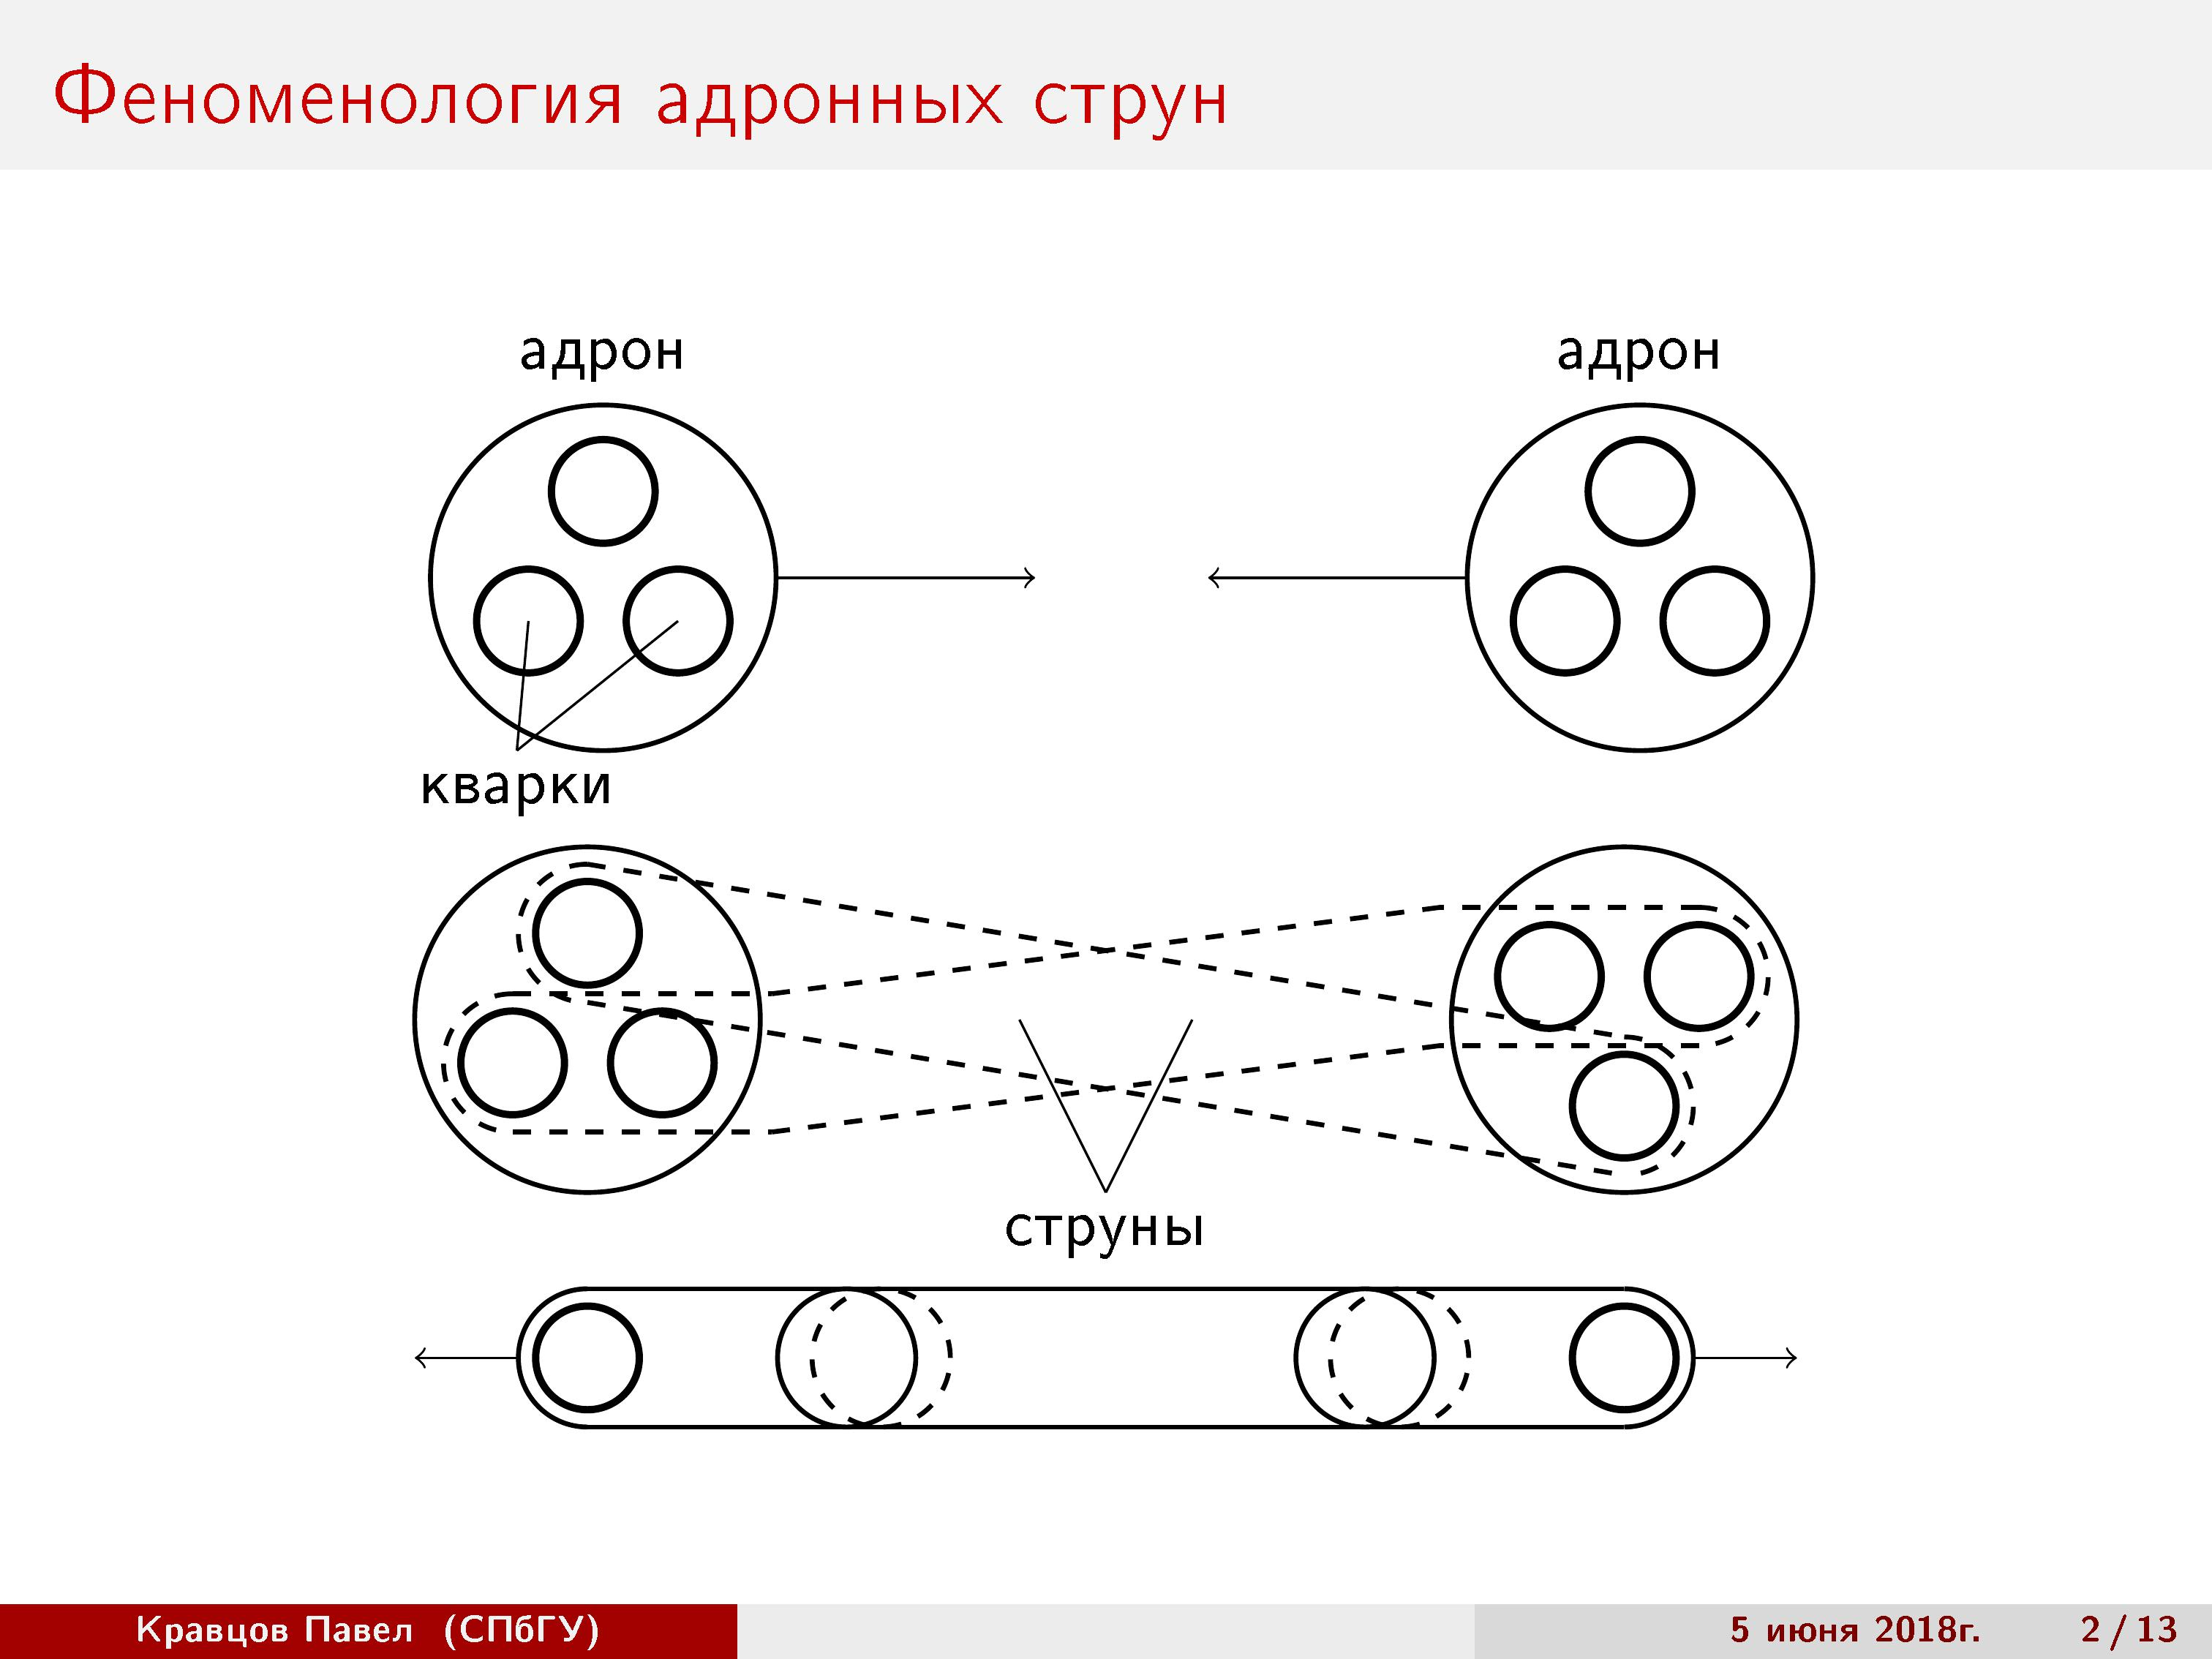
\includegraphics[width=1\linewidth]{page-02.jpg}
\end{minipage}
\begin{minipage}[h]{0.7\linewidth}
	В работе мы рассматриваем адронные столкновения в феноменологии адронных струн. Здесь механизм столкновения представляется следушим образом:
	\begin{itemize}
		\item Друг навстречу другу летят адроны с околосветовой скоростью.
		\item Они состоят из кварков.
		\item Цветовые поля кварков перецепляются на кварки другого адрона и образуются т. н. струны.
		\item Струны представляют собой трубки цветового поля с разлетаюшимися на концах кварками
		\item В струнах запасена энергия, достаточная для образования множества частиц, поэтому они каскадно рвутся на более мелкии струны.
	\end{itemize}
\end{minipage}
\line

\begin{minipage}[h]{0.39\linewidth}
	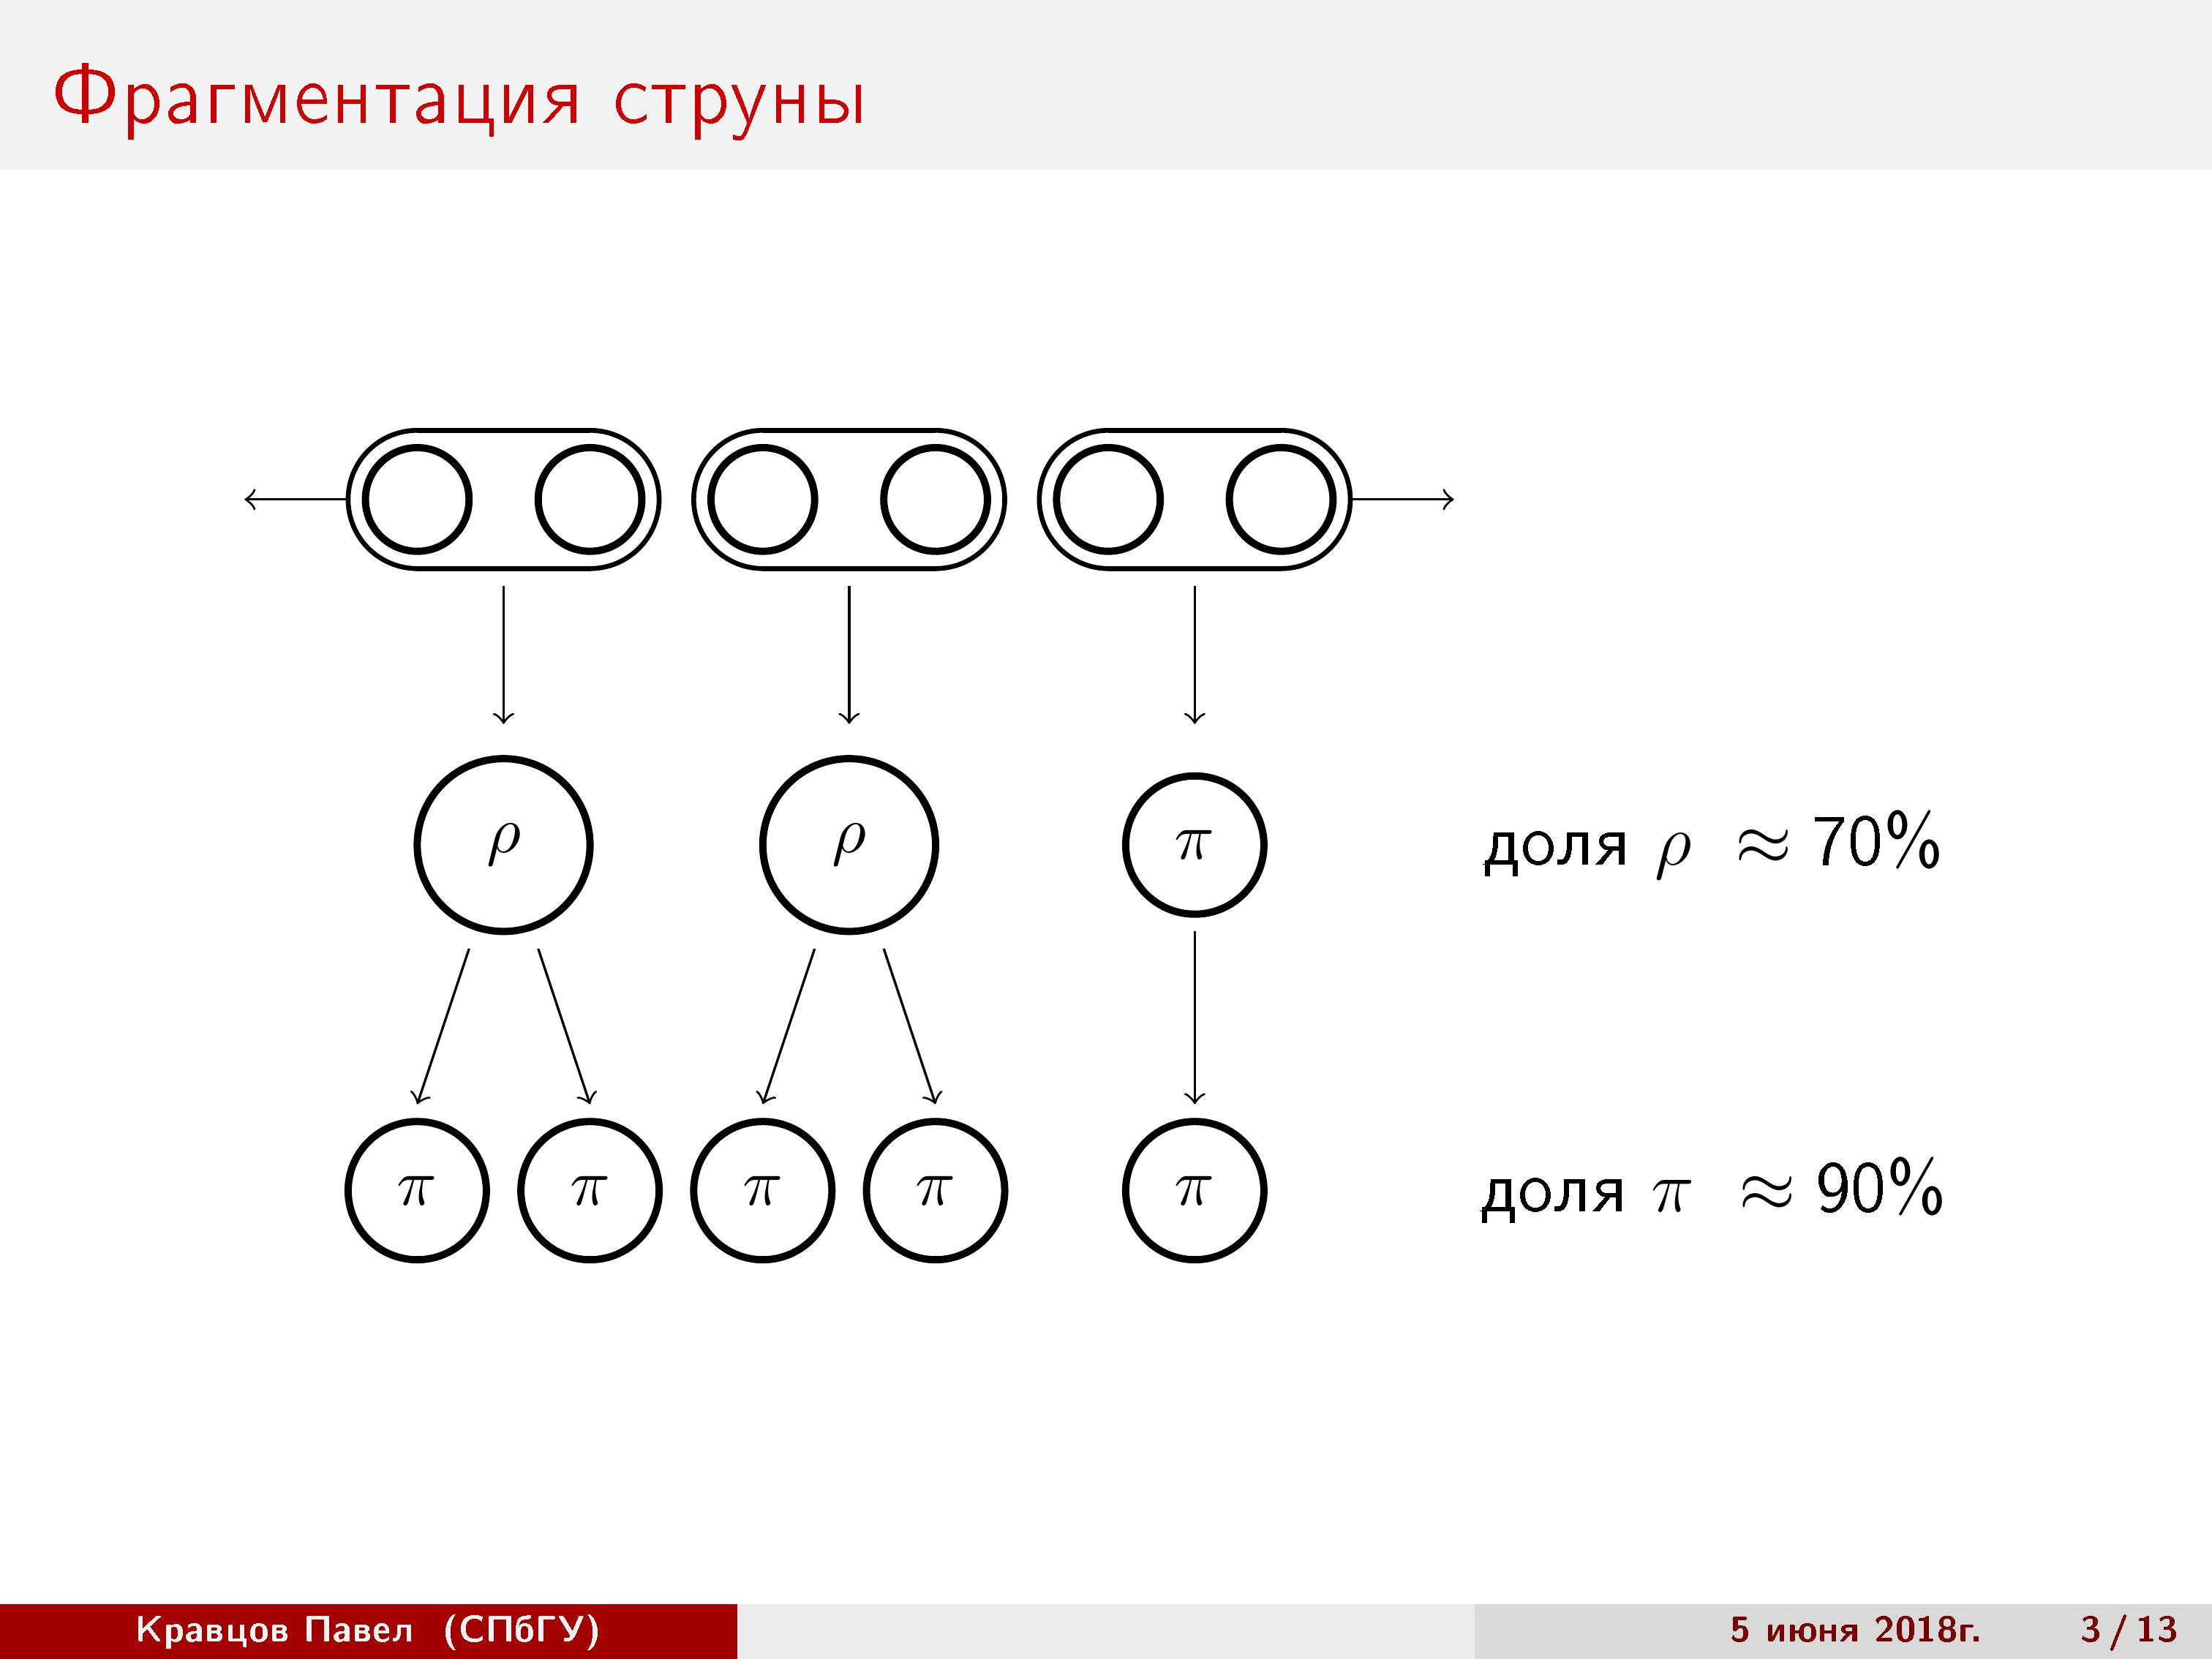
\includegraphics[width=1\linewidth]{page-03.jpg}
\end{minipage}
\begin{minipage}[h]{0.6\linewidth}
	\begin{itemize}
		\item Фрагменты струны, которые слишком малы для дальнейшего деления, в данной феноменологии представляются новыми частицами с соответствуюшим кварковым составом.
		\item До детекторов доходит множество частиц, более 90\% из них - пионы.
		\item Тем не менее считается что большинство \p-мезонов образовались не непосредственно из струн, а от распадов \ro-мезонов, которые появились от фрагментации струны.
	\end{itemize}
\end{minipage}
\line

\begin{minipage}[h]{0.29\linewidth}
	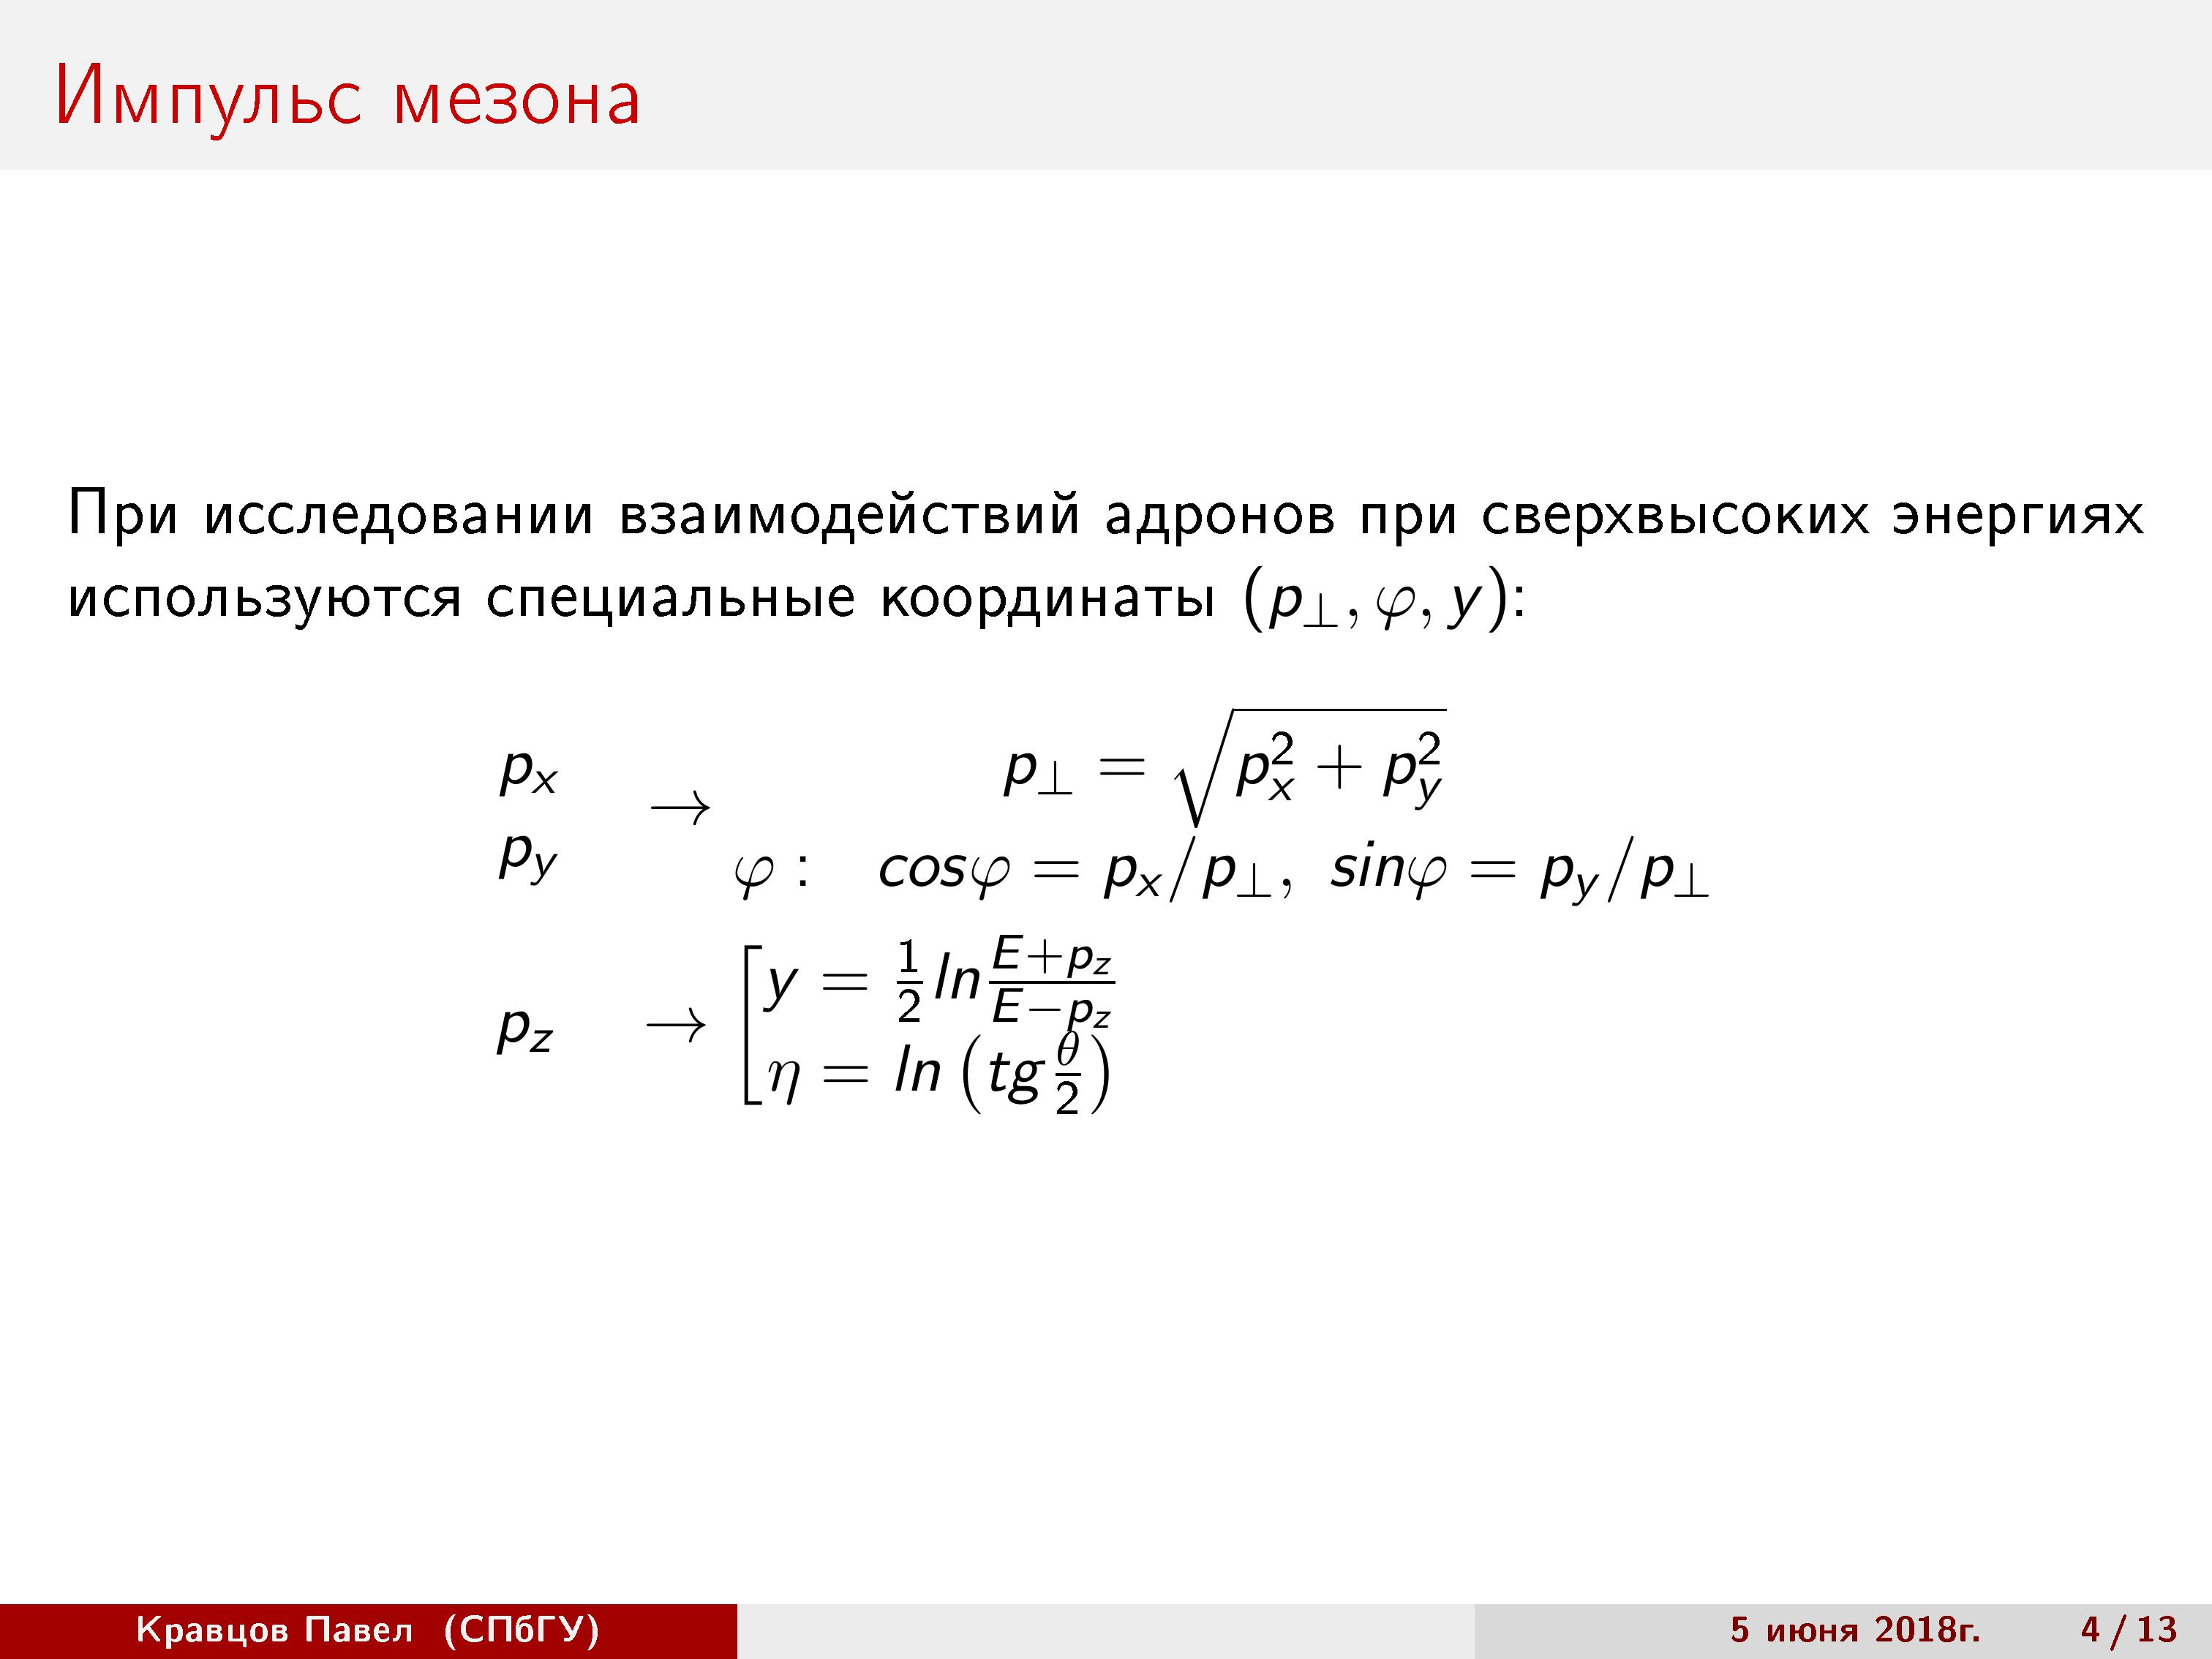
\includegraphics[width=1\linewidth]{page-04.jpg}
\end{minipage}
\begin{minipage}[h]{0.7\linewidth}
	Для исследования столкновений при сверхвысоких энергиях используются специальные координаты. Мы считаем ось z соноправленной с осью столкновения. Если у нас есть частица с декартовыми компонентами $p_x, p_y, p_z$, то вместо $p_x, p_y$ мы вводим полярные координаты - поперечный импульс и азимутальный угол. \\
	\qquad Вместо z-компоненты используестя либо быстрота, которая выражается через энергию частицы и z-компоненту импульса, либо псевдобыстрота, которая зависит от угла между импульсом и осью z. Псевдобыстрота больше подходит для экспериментальных данных, т. к., для ее определения, нужно знать лишь направление движения. На самом деле эти велечины приблизительно равны друг другу.
\end{minipage}
\line

\begin{minipage}[h]{0.29\linewidth}
	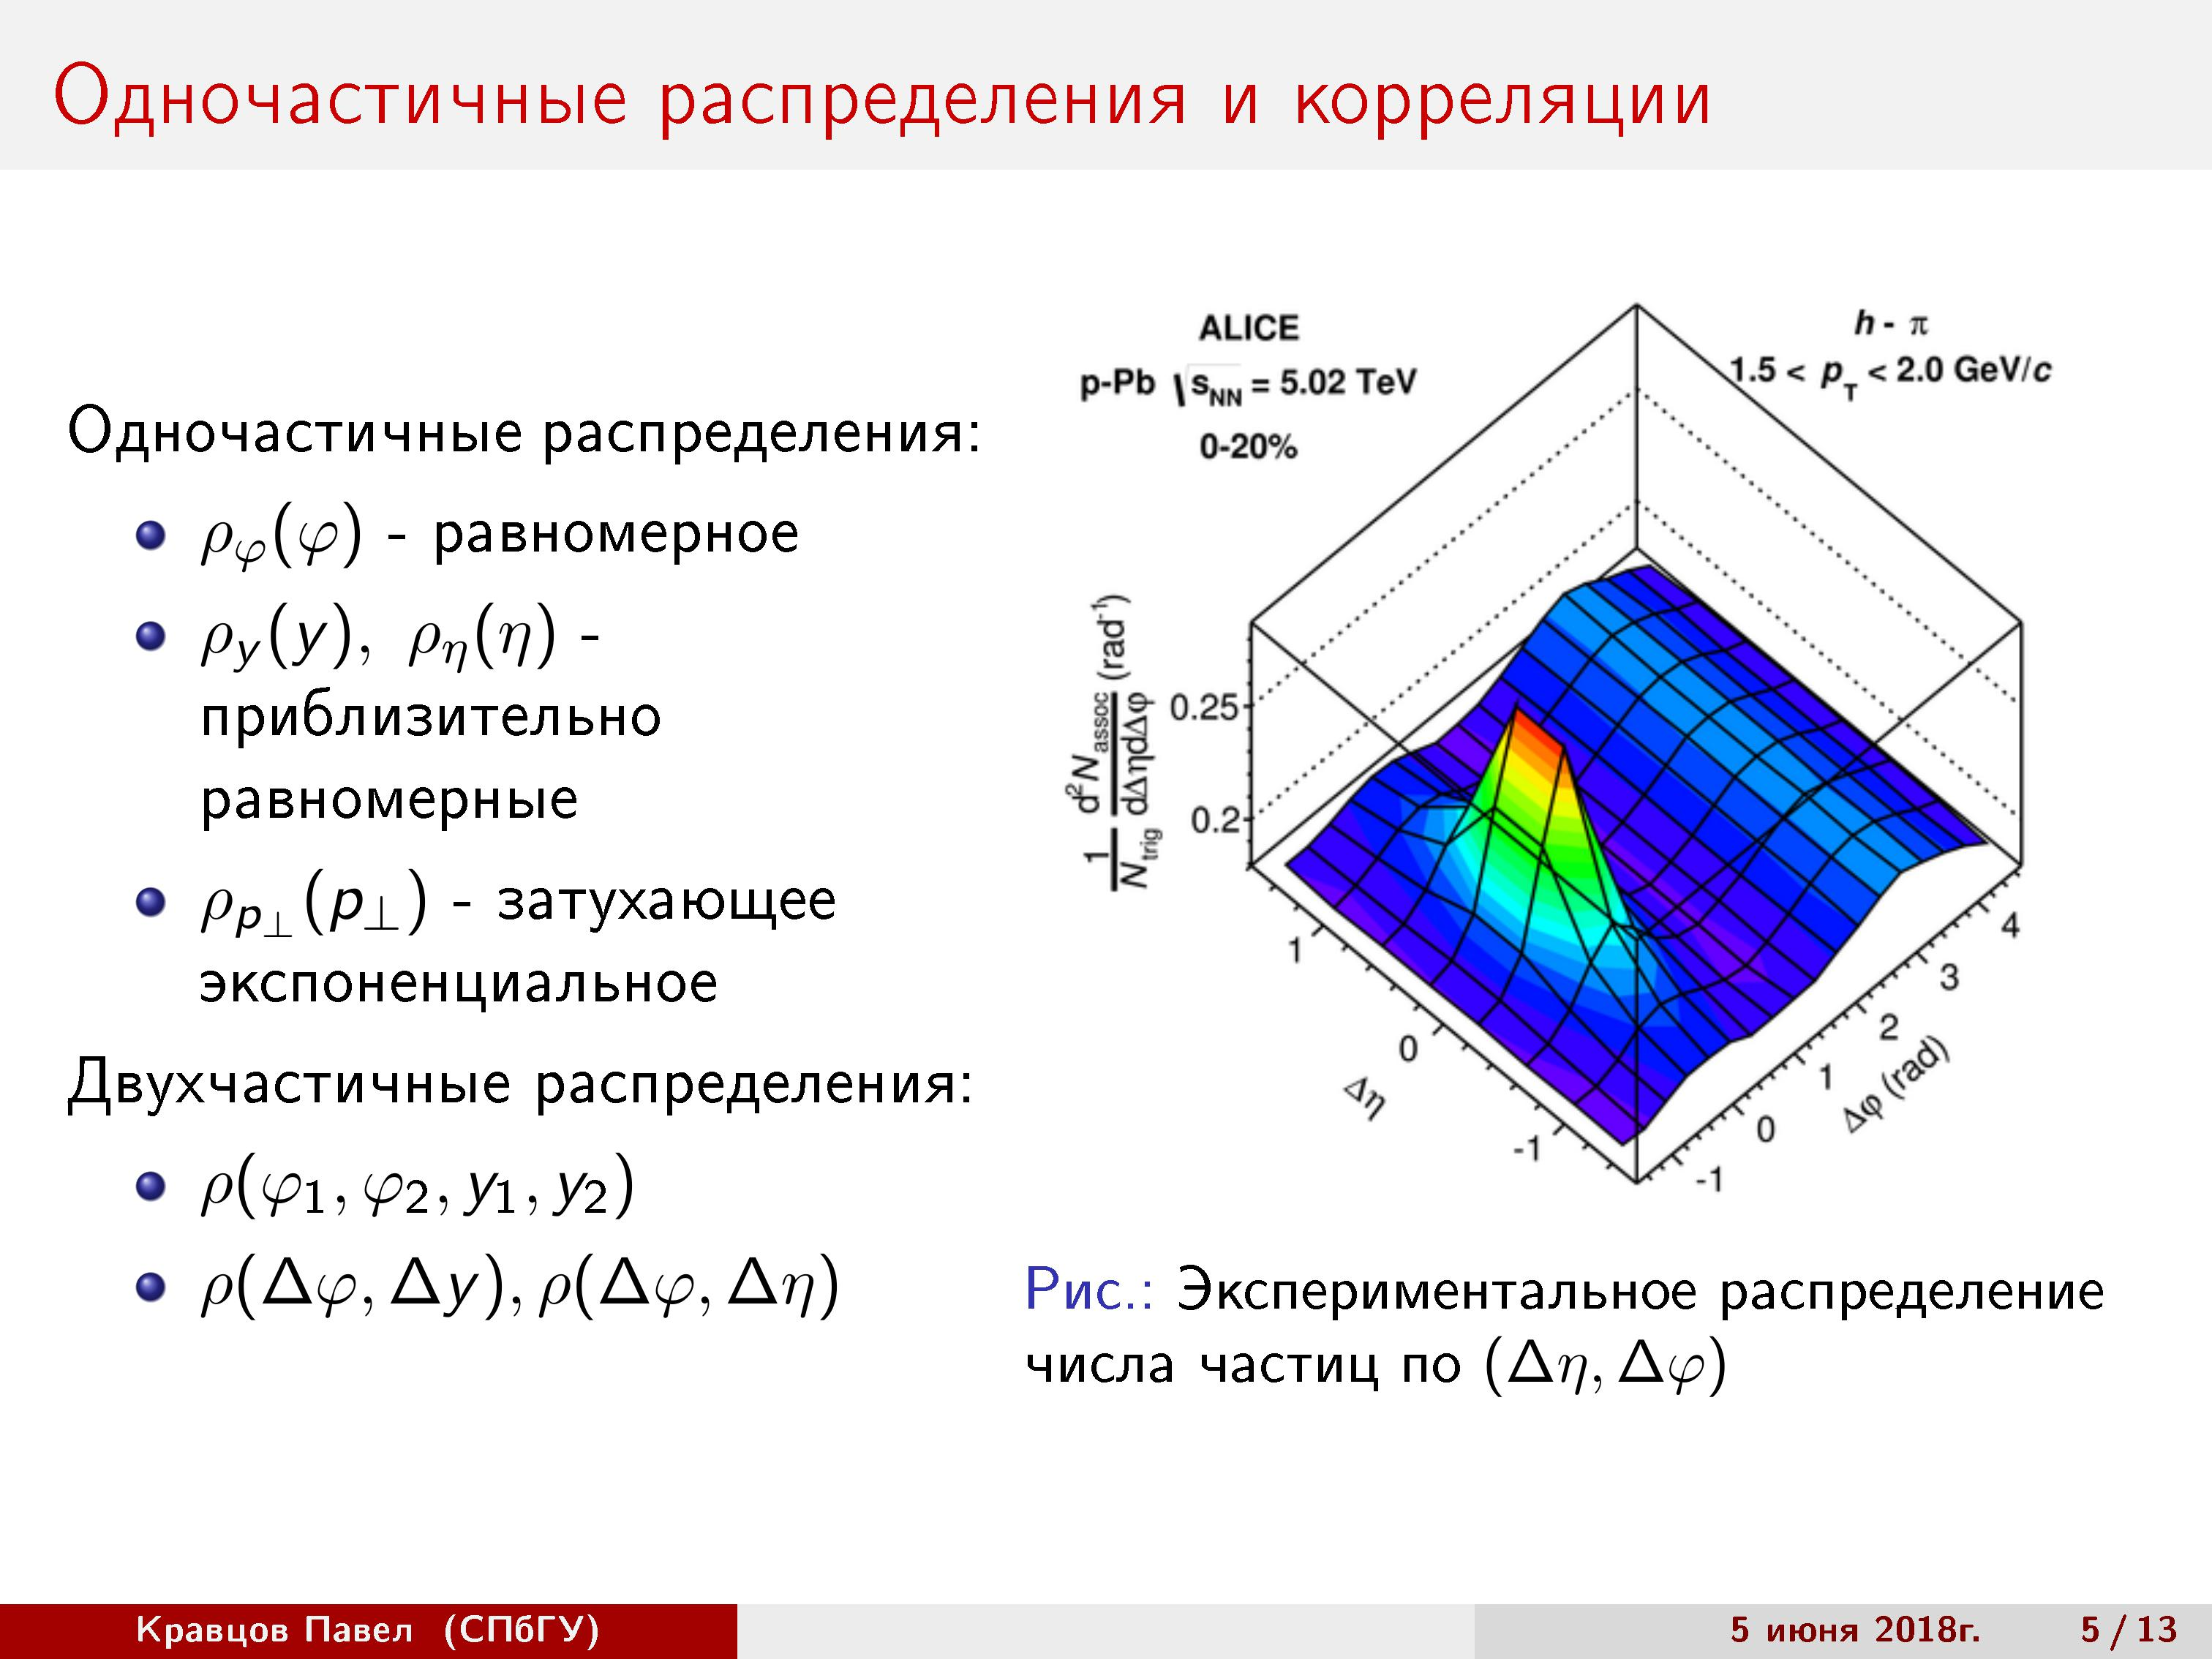
\includegraphics[width=1\linewidth]{page-05.jpg}
\end{minipage}
\begin{minipage}[h]{0.7\linewidth}
	Итак, по азимутальному углу, быстроте и поперечному импульсу рассматривают распределения частиц. Мы обозначаем через $\rho$ - плотность распределения, и если необходимо ставим индекс. Про распределения известно следушее:
	\begin{itemize}
		\item Из симметрии вокруг оси z распределение по азимутальному углу $\phi$ равномерно.
		\item Из эксперимента также известно, что распределения по быстроте и псевдобыстроте приблизительно равномерное в широком диапазоне.
		\item Про импульс известно, что он экспоненциально убывает.
		Это все что можно сказать про одночастичные распределения.
	\end{itemize}
	\qquad Более содержательными являются двухчастичные распределения или корреляции. Мы смотрим на распределения компонент импульса у пары частиц. То есть на функции вроде этой. Так как распределения по углу $\phi$ и быстроте равномерны, то нетривиальная зависимость может получится лишь по разности компонент. Поэтому обычно рассматривают двумерное распределение Зависящее от разности углов и разности быстрот. Ну или псевдобыстрот. На рис типичное распределение по азимутальному углу и псевдобыстроте, полученное из эксперимента.
\end{minipage}
\line

\begin{minipage}[h]{0.39\linewidth}
	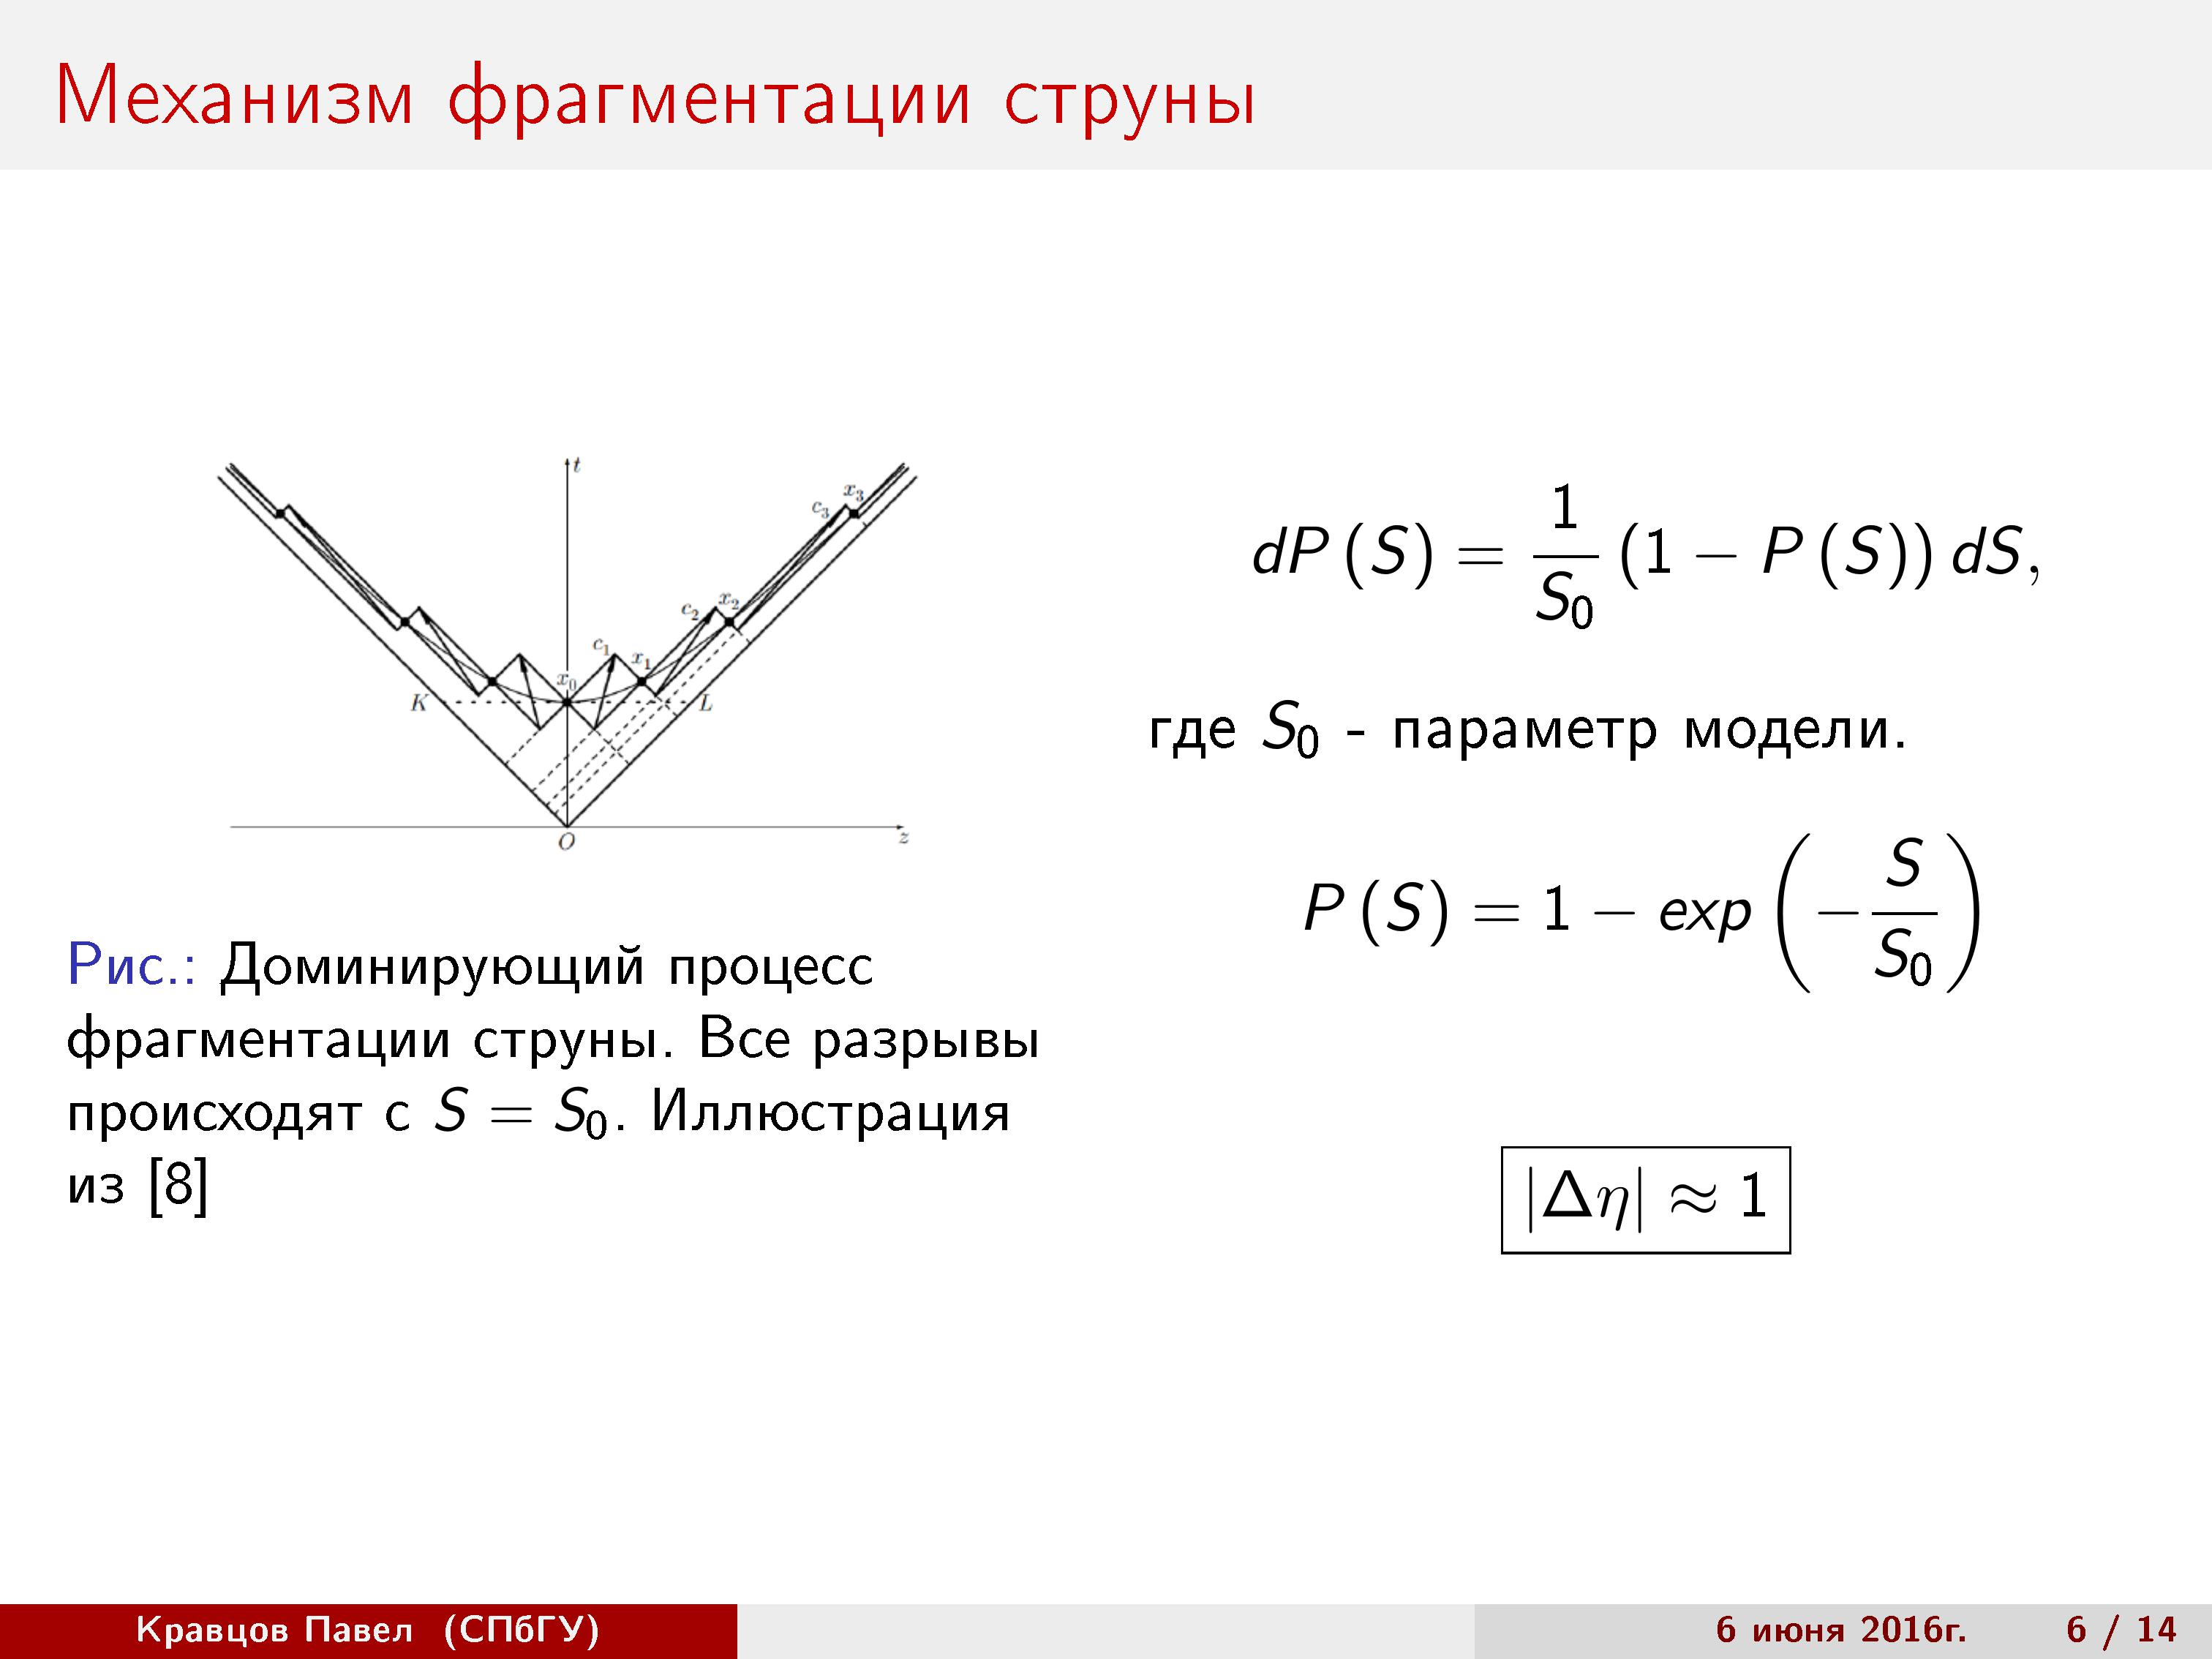
\includegraphics[width=1\linewidth]{page-06.jpg}
\end{minipage}
\begin{minipage}[h]{0.6\linewidth}
	Теперь о целях работы:
	Есть общая цель: построить простую модель на основе струнной феноменологии для объяснения поведения $(\Dphi, \Dy)$ - корреляций. Найти аналитический вид зависимости $\rho(\Dphi, \Dy)$. \\
	\qquad И есть конкретная цель для магистерской работы - это построить модель объясняющую передний пик в  распределении $\rho(\Dphi, \Dy)$ и найти формулу для него. На самом можно ожидать, что пик будет обусловлен распадом резонансов, т. к. при распаде образуются пары частиц летящих приблизительно в одном направлении.
\end{minipage}
\line

\begin{minipage}[h]{0.39\linewidth}
	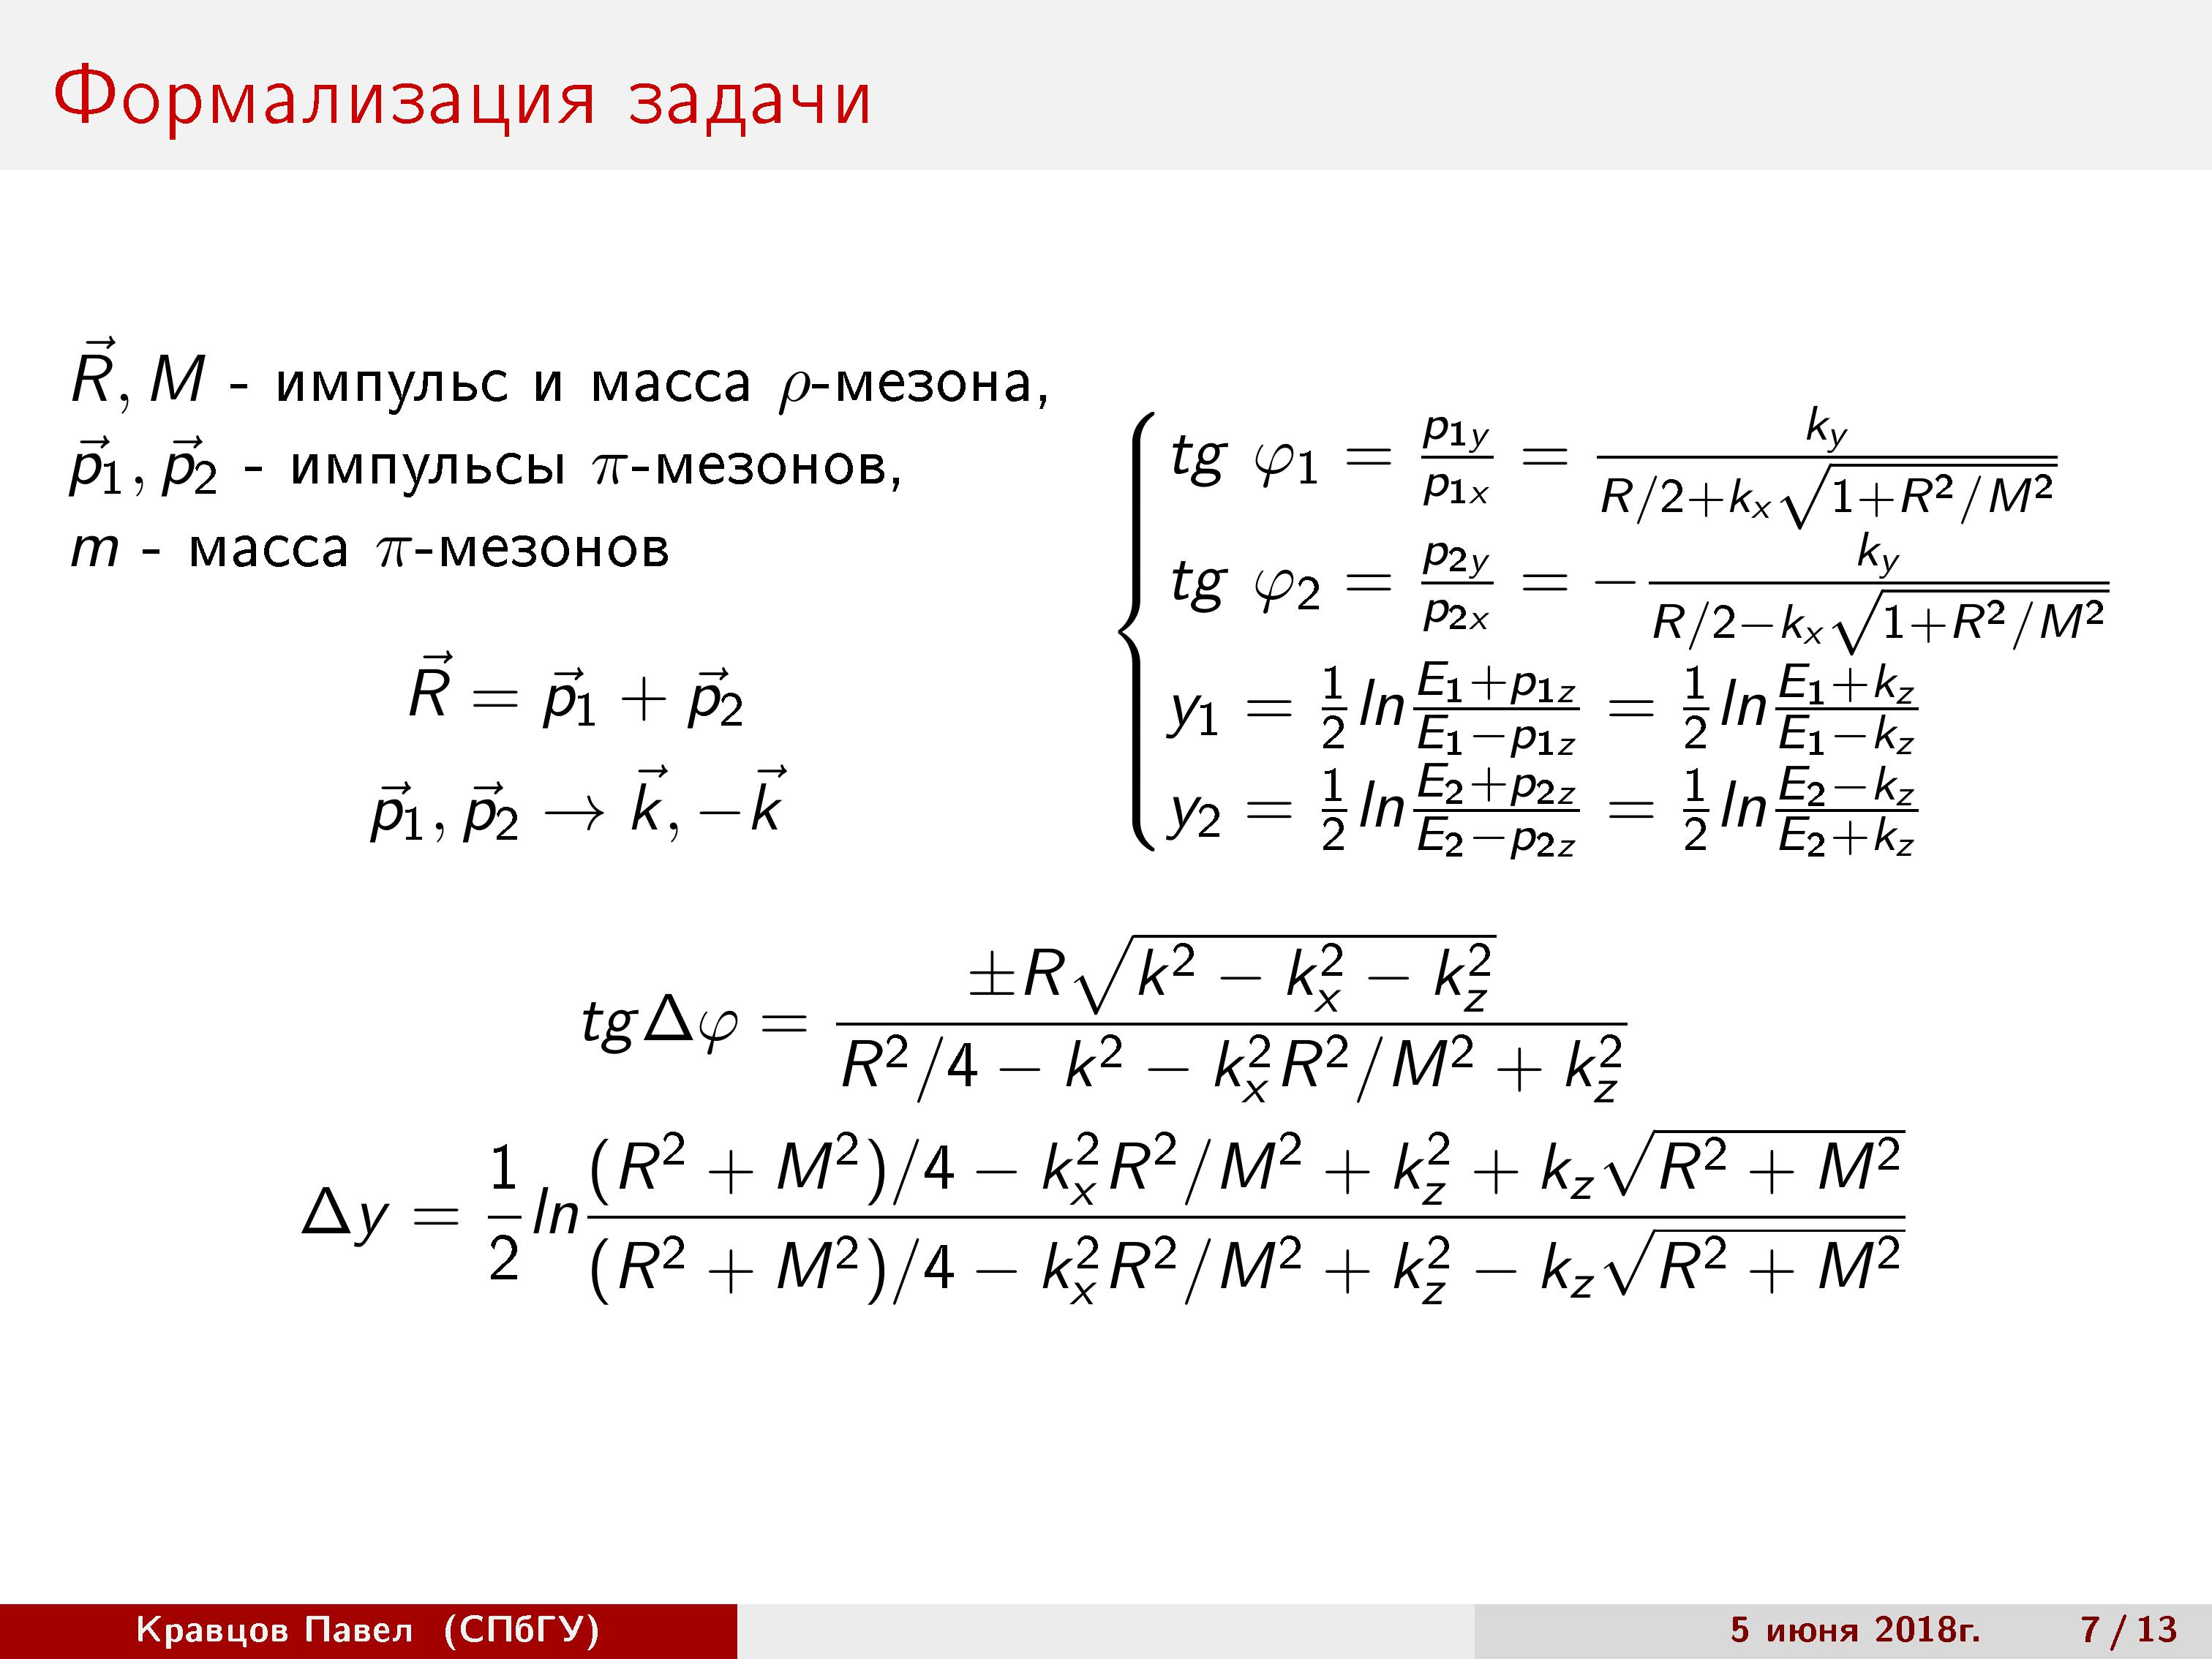
\includegraphics[width=1\linewidth]{page-07.jpg}
\end{minipage}
\begin{minipage}[h]{0.6\linewidth}
	Формализуем задачу. У нас есть \ro-мезон с импульсом R, и он распадается на 2 \p-мезона с импульсами $p_1, p_2$. В системе отсчета \ro-мезона, эти импульсы противоположны друг другу. Обозначим их k и -k. Модуль вектора k выражается через массы мезонов. Направление k мы считаем произвольным. Мы сделаем преобразования Лоренца и свяжем компоненты импульсов в разных системах отсчета. И мы можем выразить переменные $(\Dphi, \Dy)$ по которым хочется найти распределение, через переменные $(k_x, k_y, k_z)$, про которые мы знаем, что они распределены равномерно по всем направлениям. \\
	\qquad Впоследствии эту пару уравнений нужно будет обратить. Это было бы непосильной задачей, но здесь есть одинаковая комбинация, что дает шанс получить все формулы в явном виде.
\end{minipage}
\line

\begin{minipage}[h]{0.29\linewidth}
	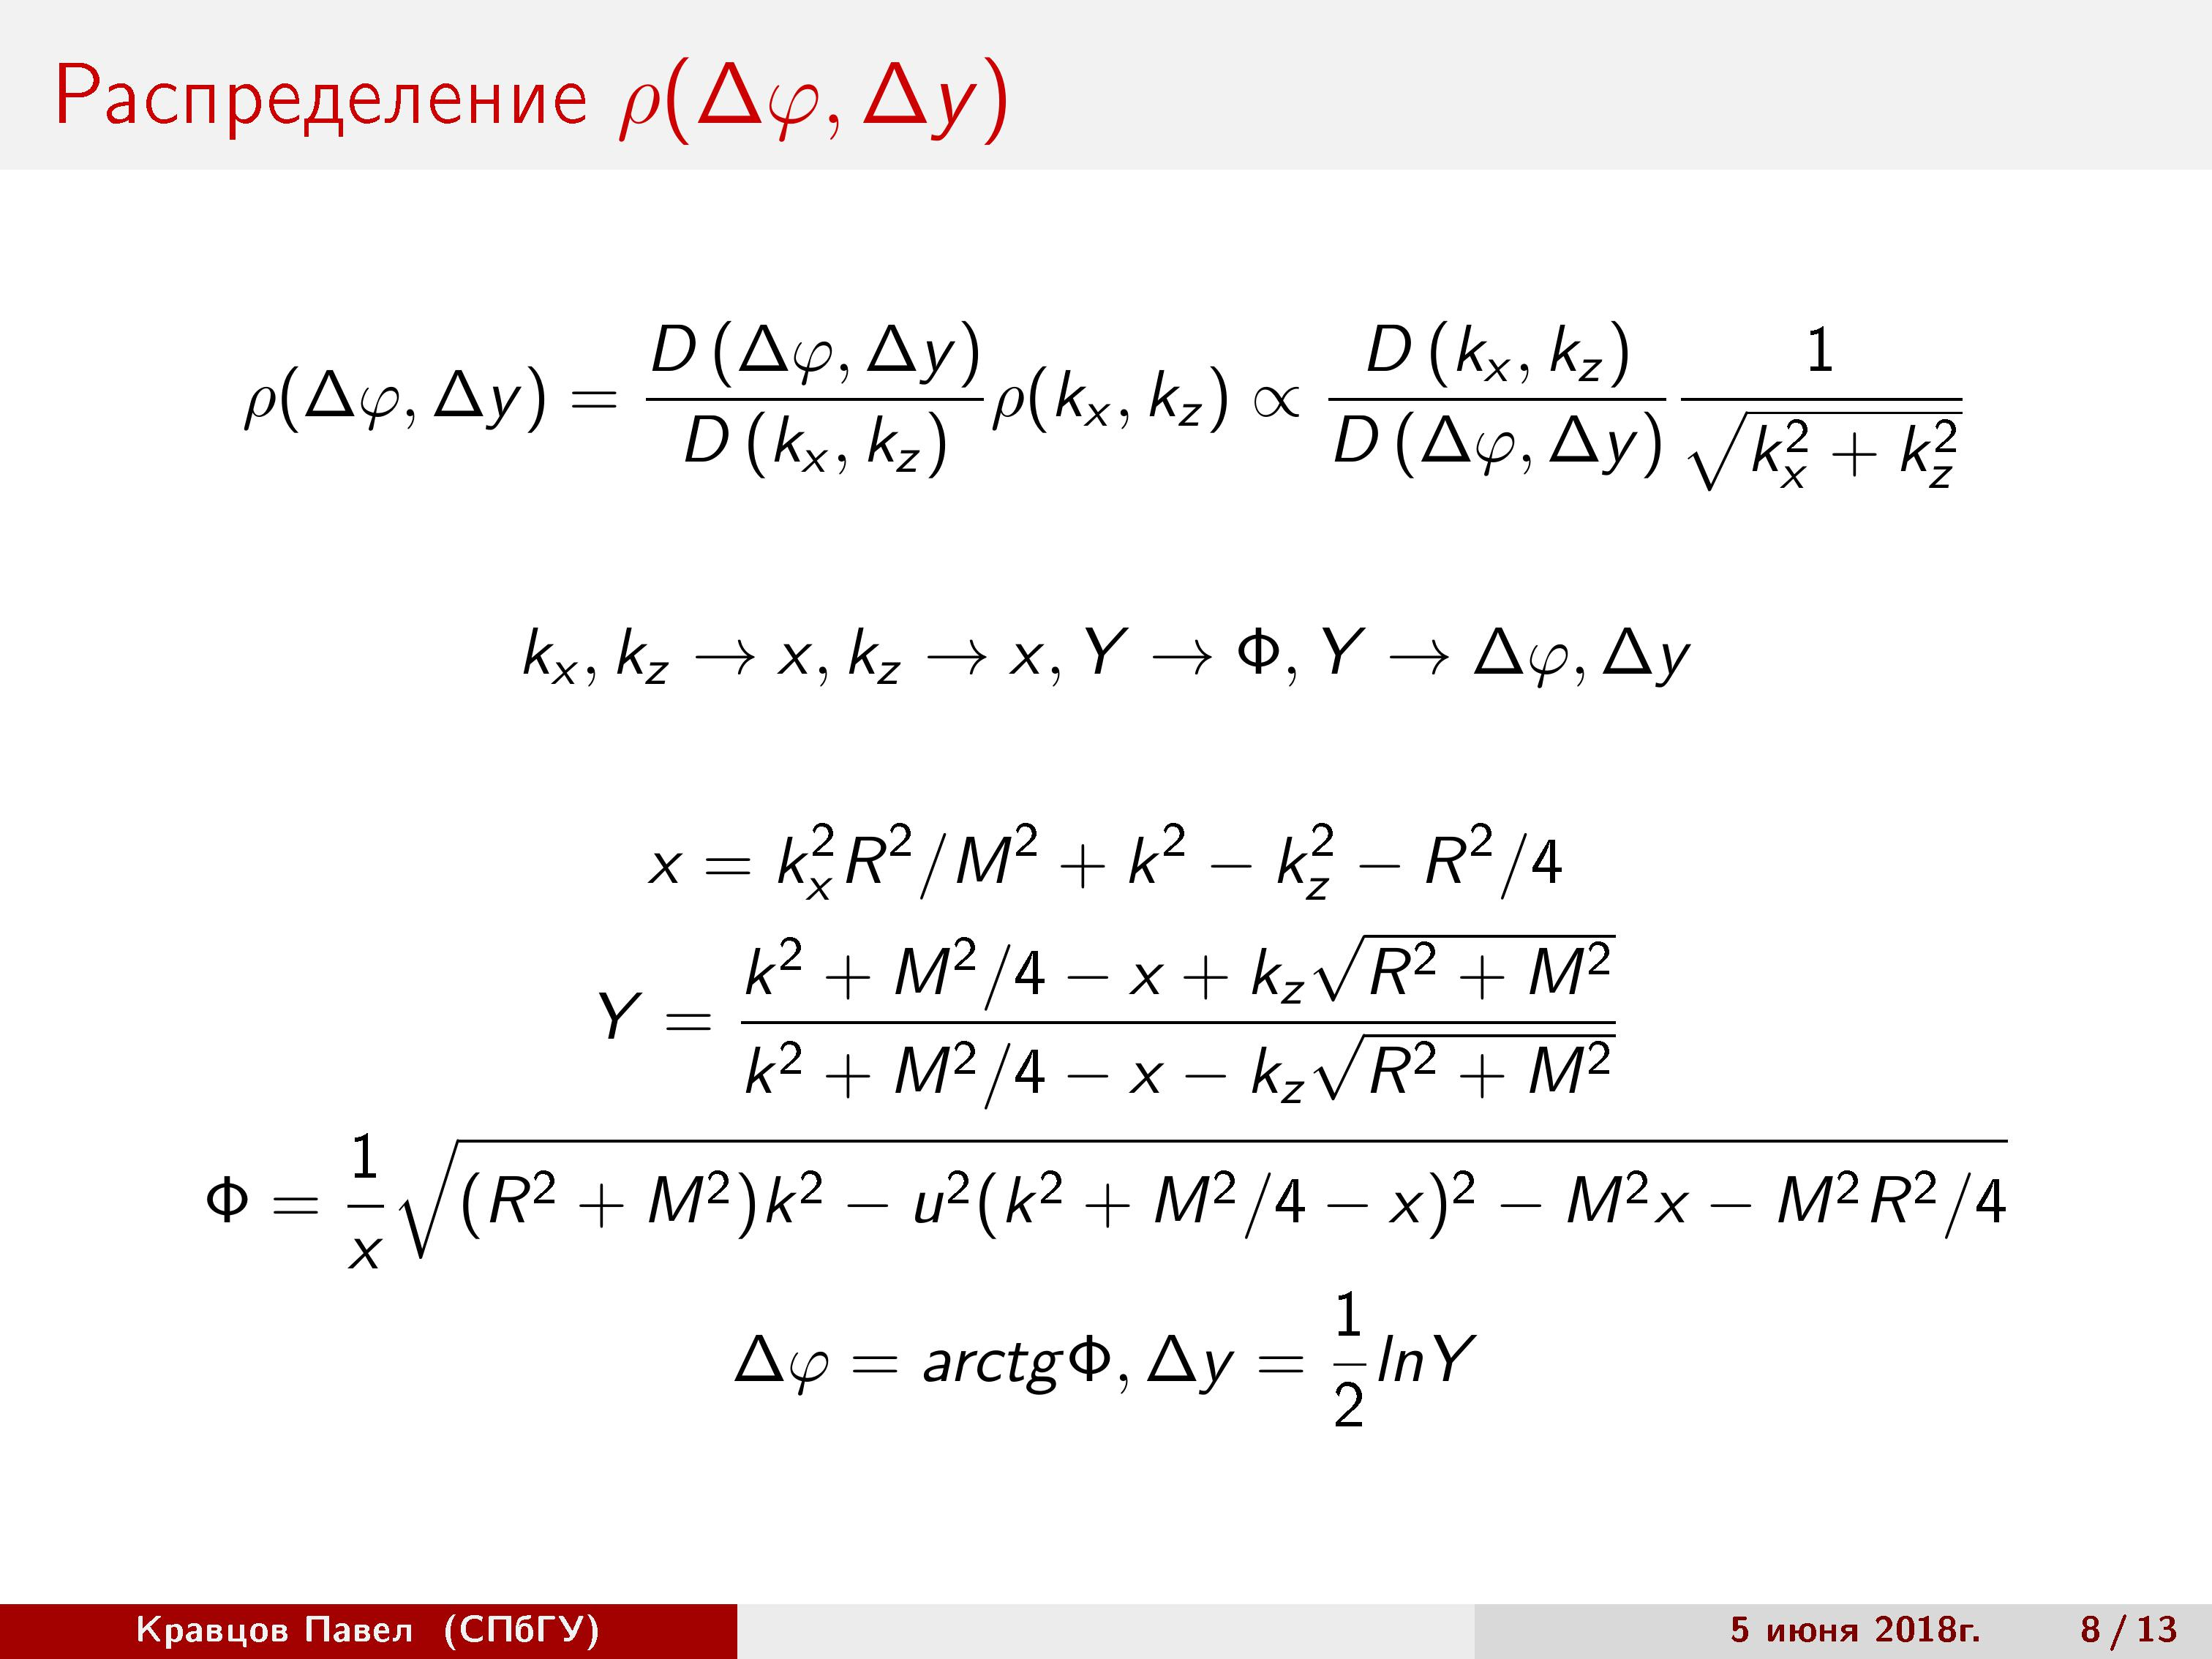
\includegraphics[width=1\linewidth]{page-08.jpg}
\end{minipage}
\begin{minipage}[h]{0.7\linewidth}
	Можно исключить из рассмотрения одну из компонент вектора k, например у-компоненту, т. к. у к фиксировваный модуль и можно выразить $k_y$, через $k_x, k_z$. Распределения связаны следующим через якобиан преобразования координат. Равномерное распределение по направлениям в декартовых координатах выглядит так. Для вычисления определителя мы делаем поочередную замену координат.
\end{minipage}
\line

\begin{minipage}[h]{0.29\linewidth}
	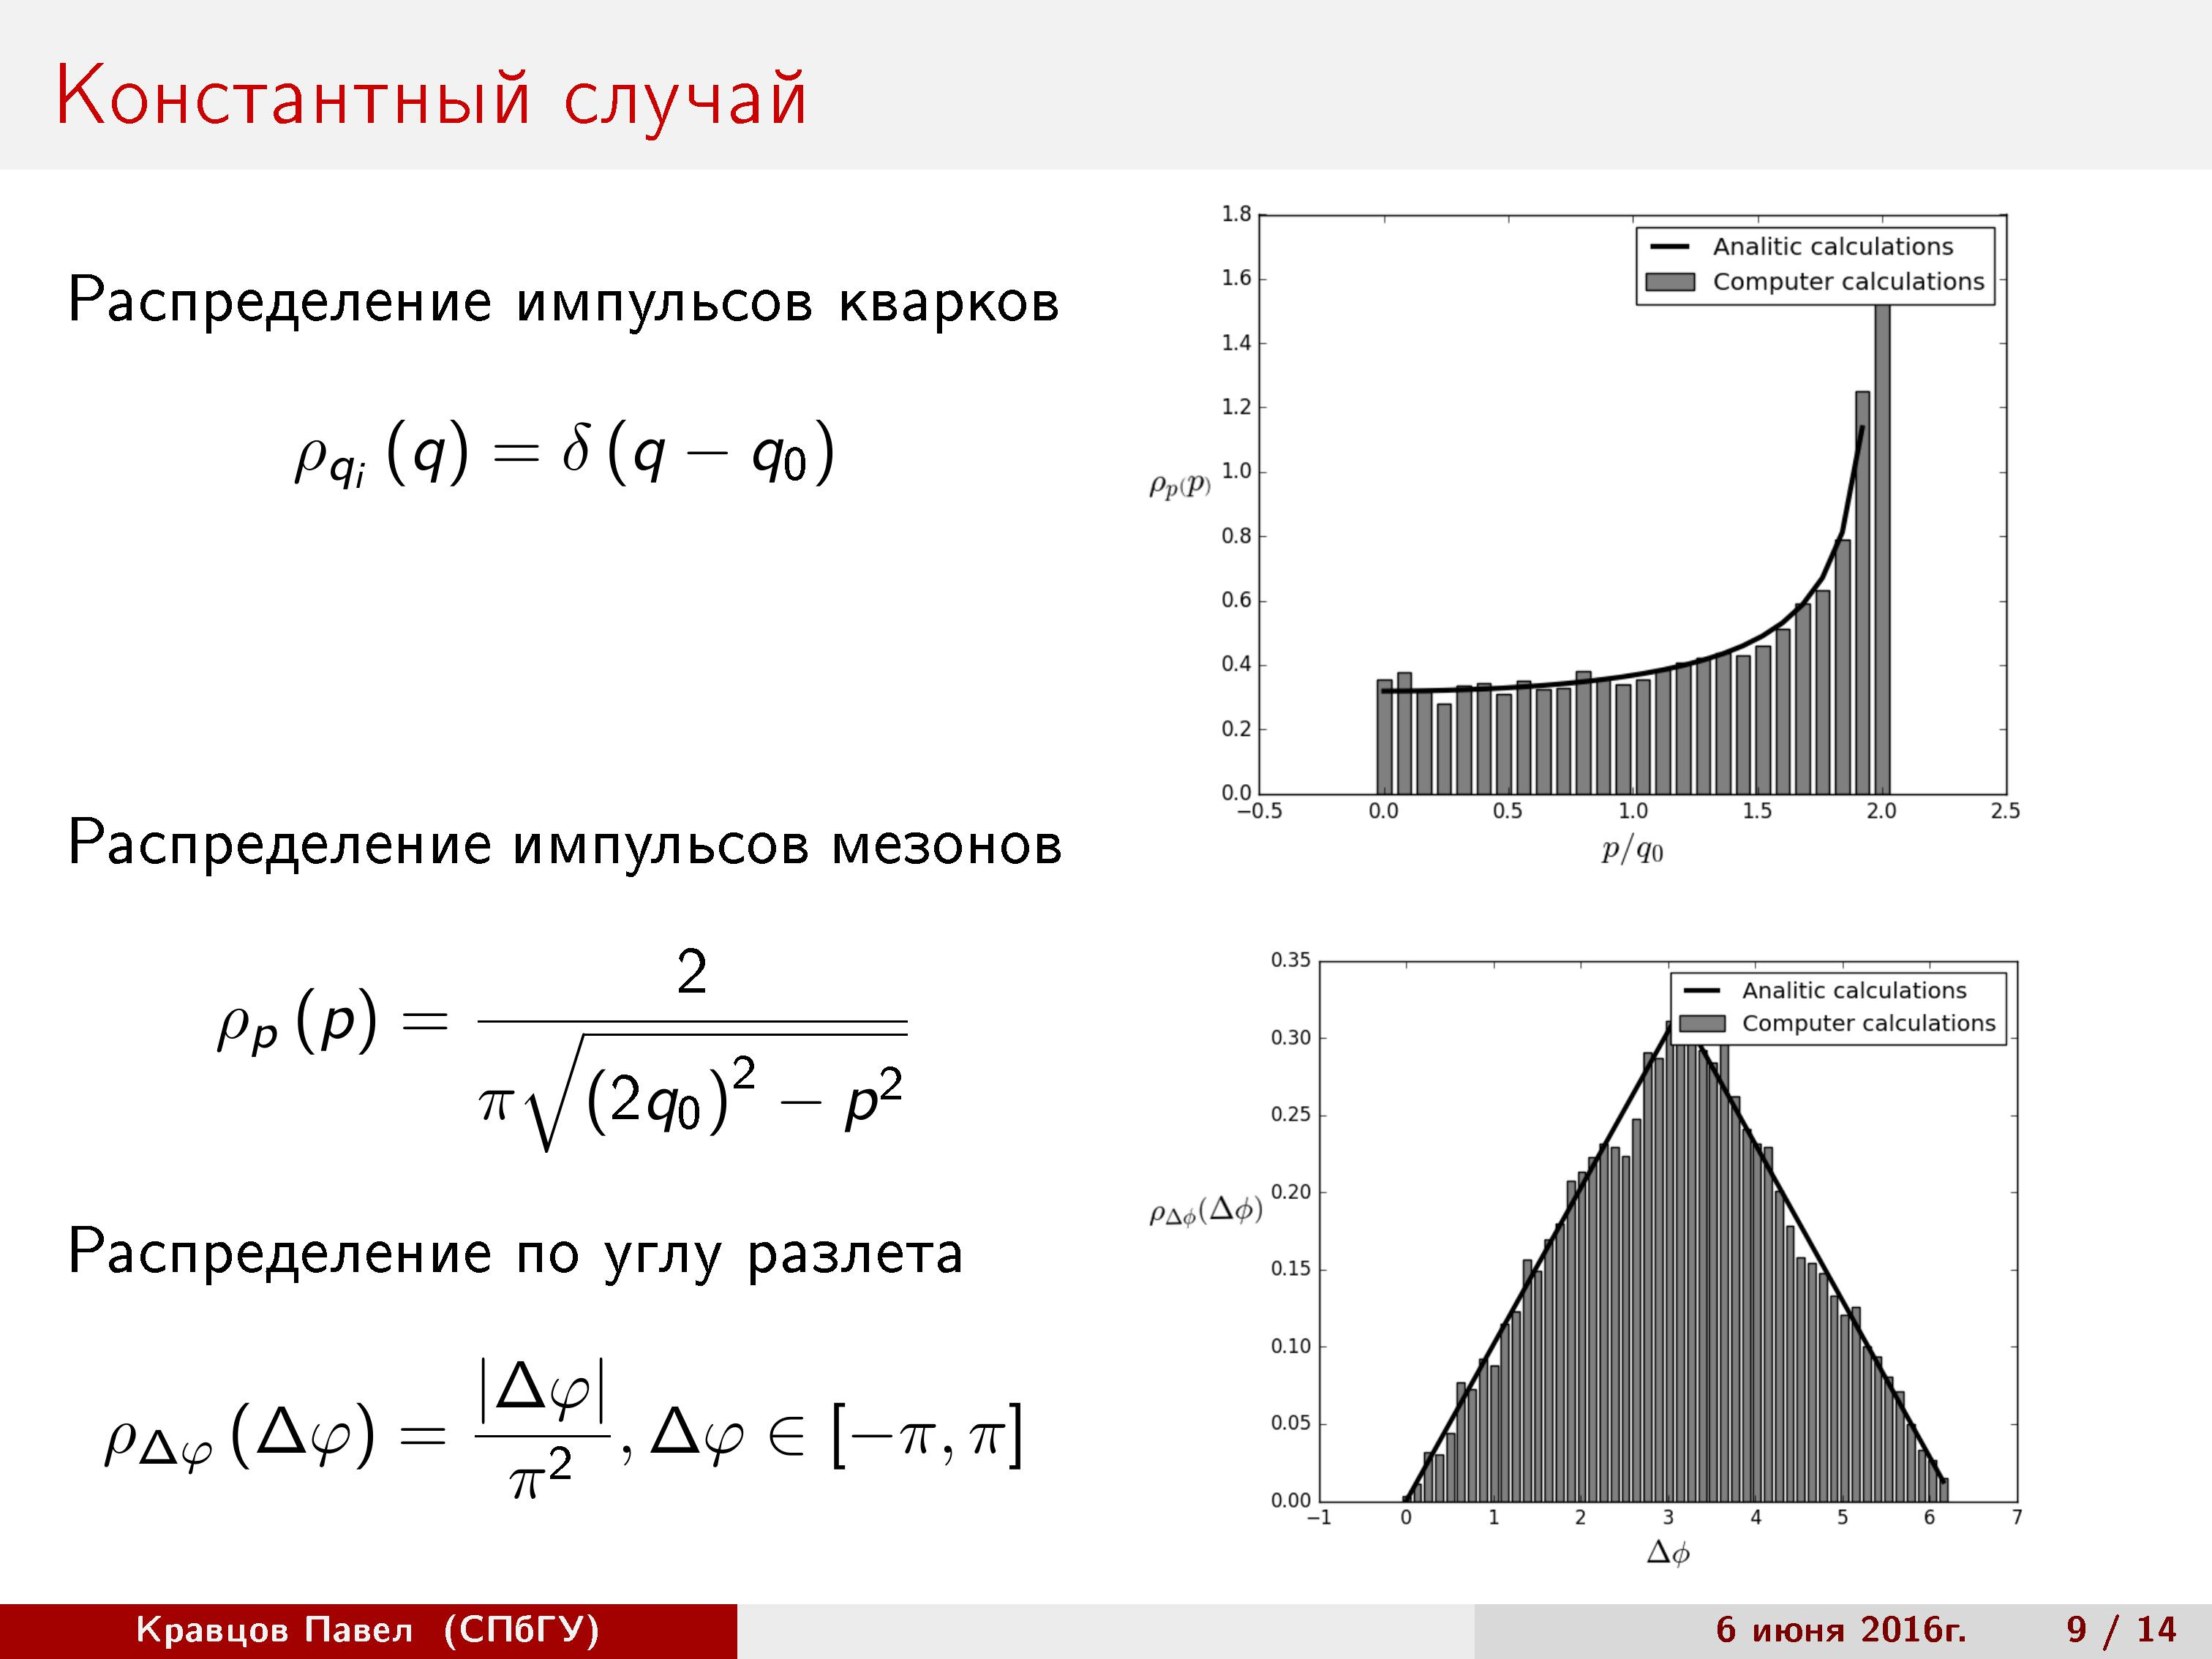
\includegraphics[width=1\linewidth]{page-09.jpg}
\end{minipage}
\begin{minipage}[h]{0.7\linewidth}
	Определитель представляется как произведение определителей, и все сводится к вычислению частных производных. Окончательные выражения очень громоздки, тем не менее ответ получается в виде явной формулы.
\end{minipage}
\line

\begin{minipage}[h]{0.29\linewidth}
	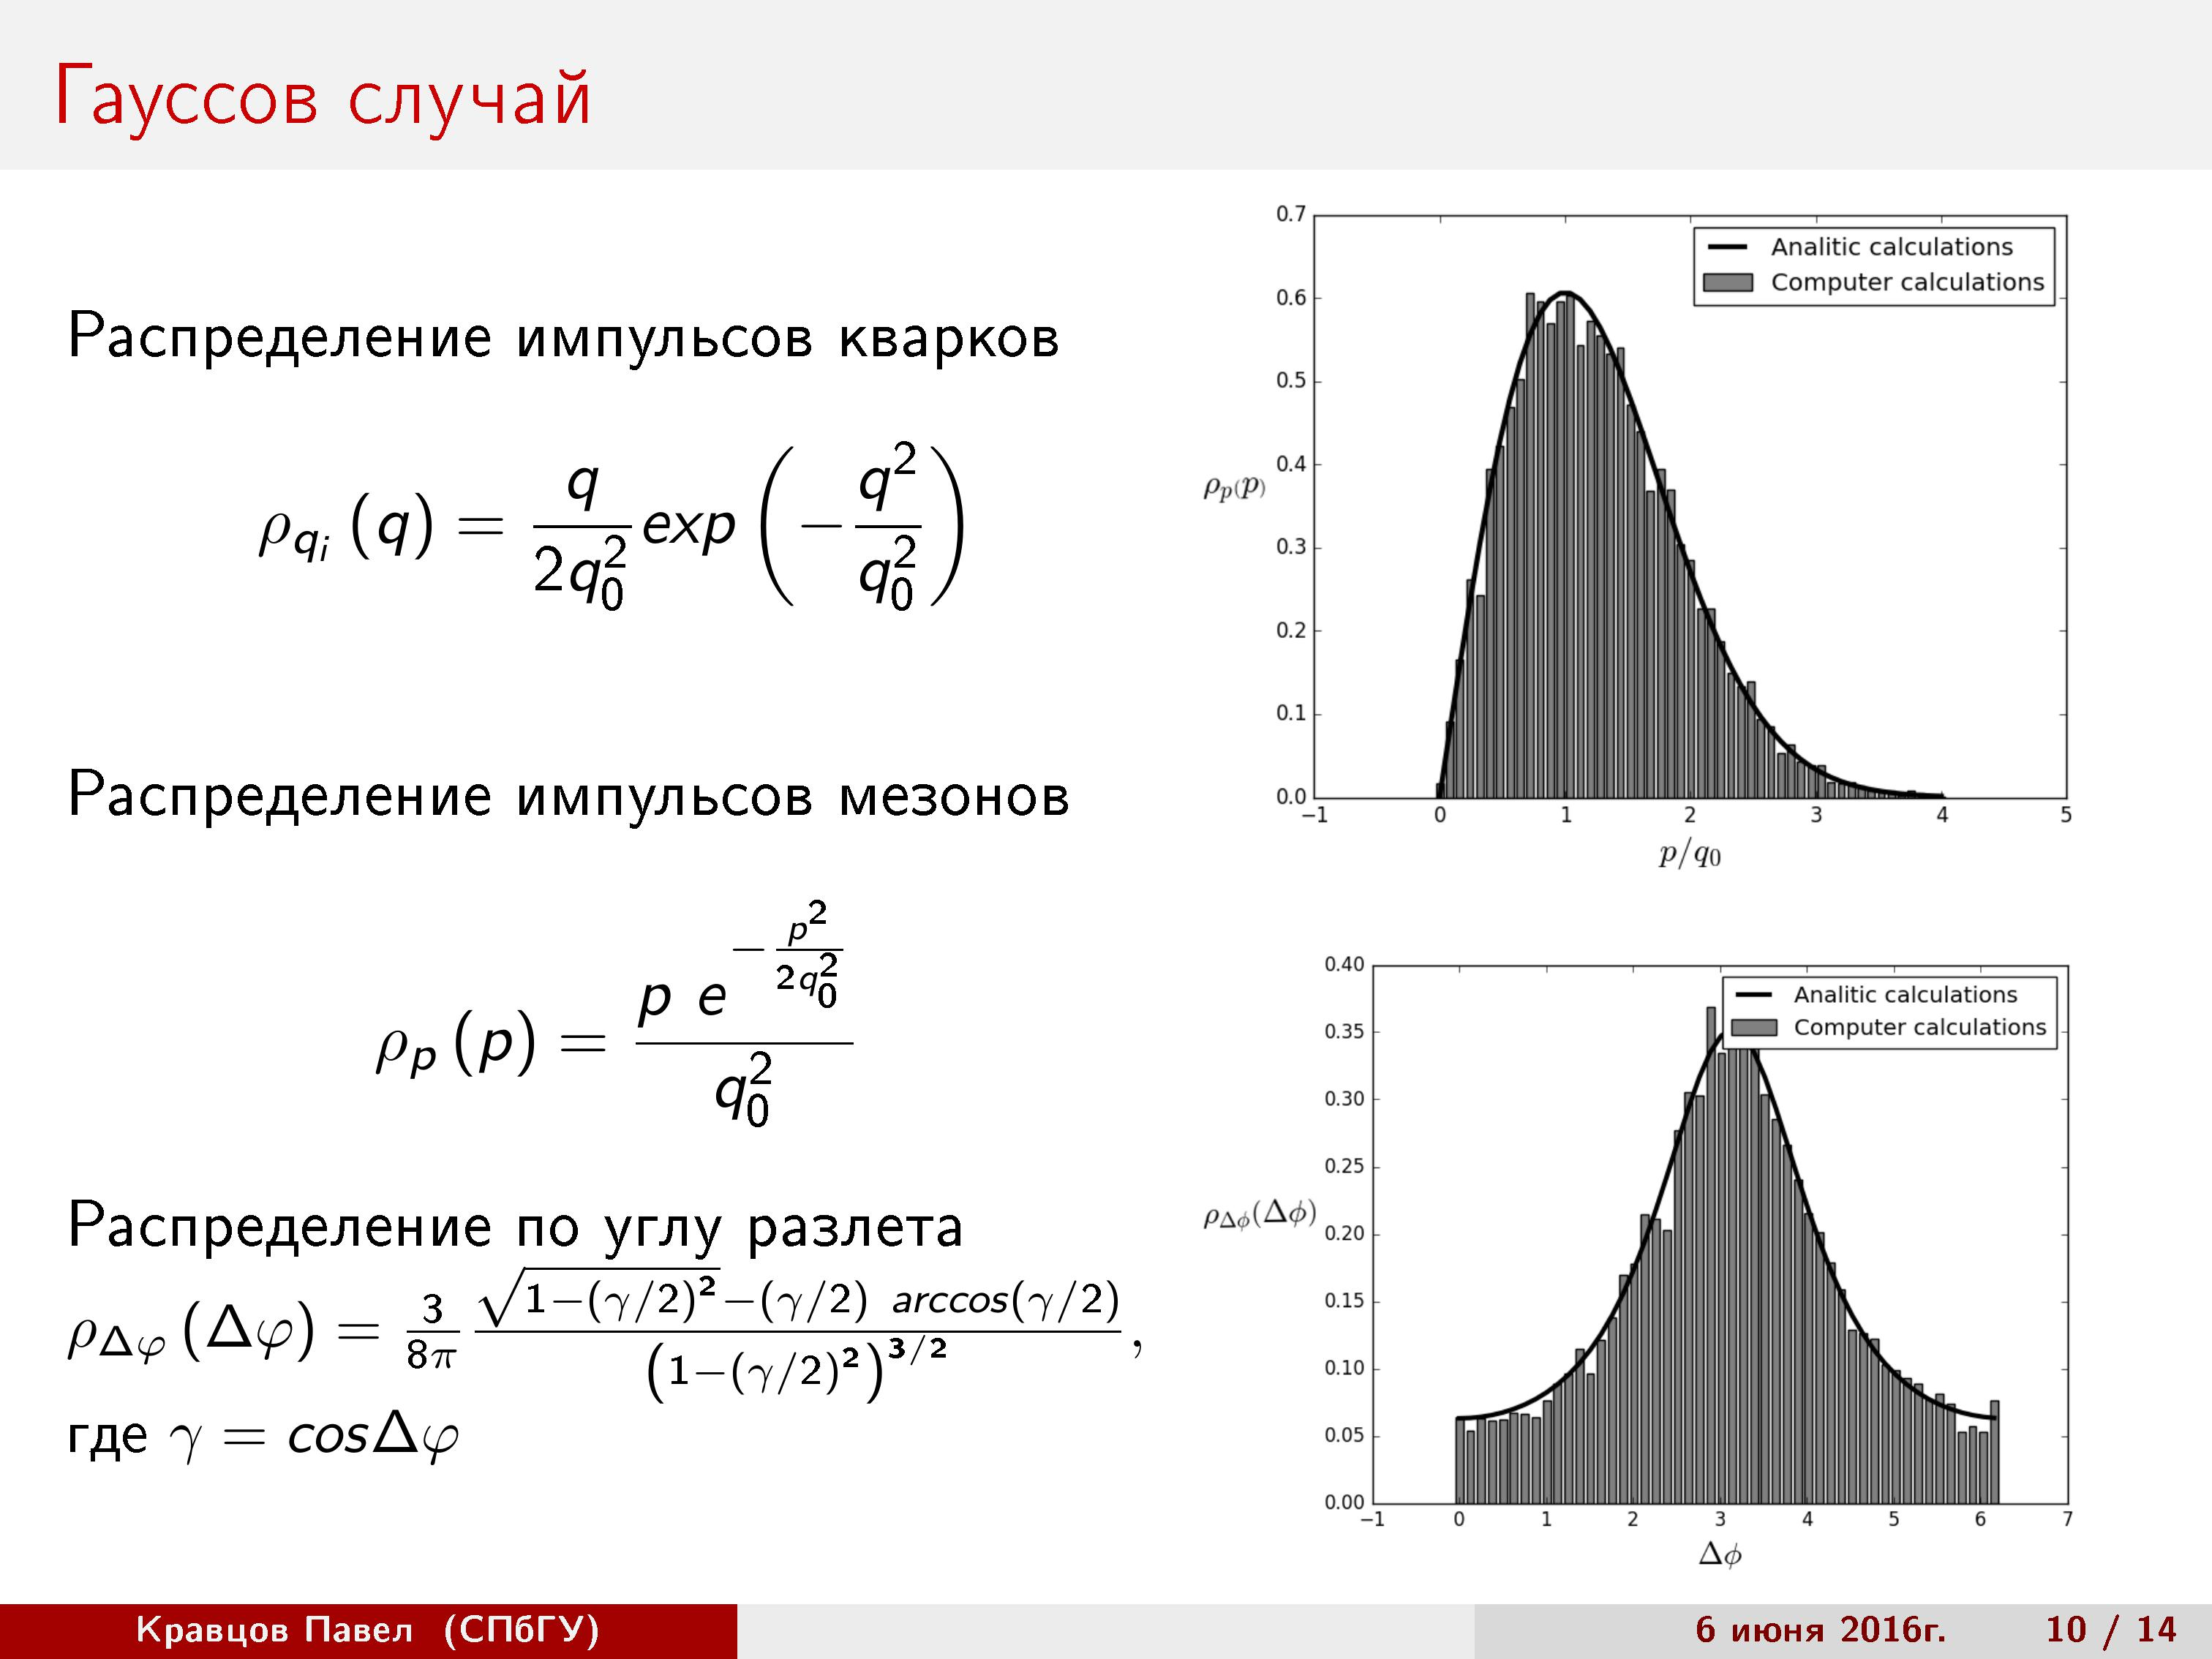
\includegraphics[width=1\linewidth]{page-10.jpg}
\end{minipage}
\begin{minipage}[h]{0.7\linewidth}
	На графиках представлен результат вычислений в графической форме. Результат зависит от модуля импульса \ro-мезона R. Если он большой то виден явный пик, если маленький, то пик разделяется надвое.
\end{minipage}
\line

\begin{minipage}[h]{0.29\linewidth}
	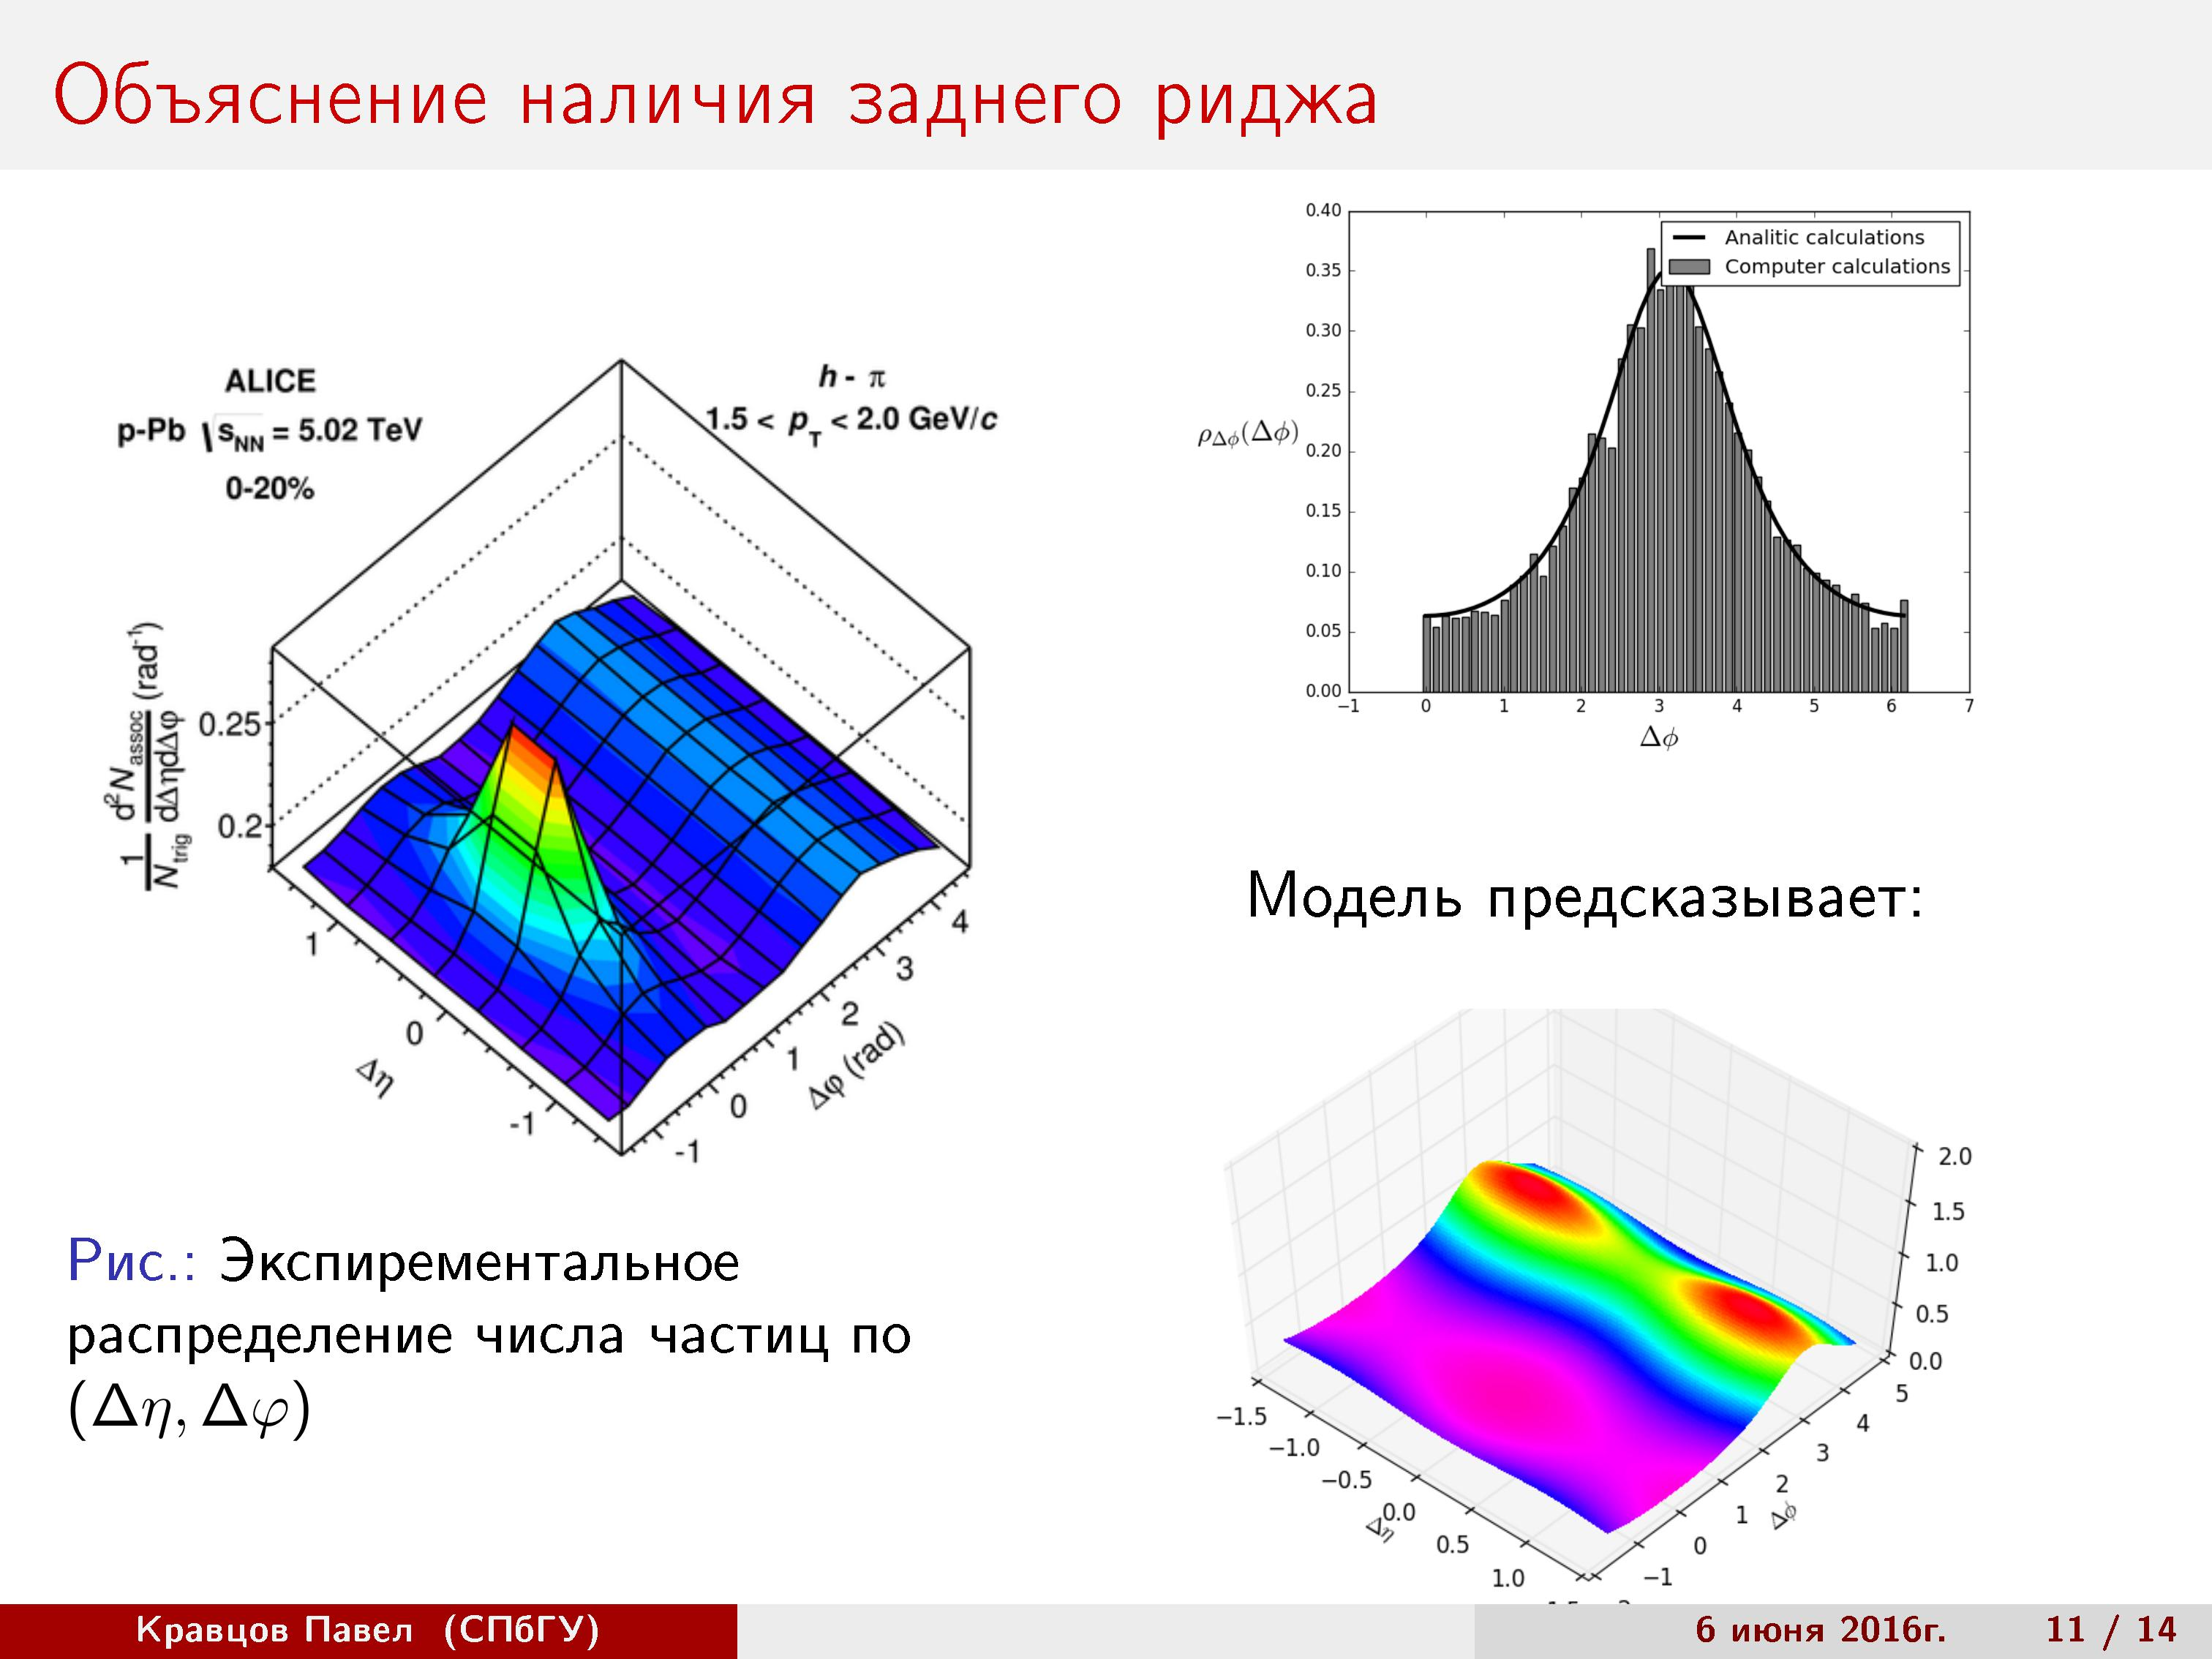
\includegraphics[width=1\linewidth]{page-11.jpg}
\end{minipage}
\begin{minipage}[h]{0.7\linewidth}
	Можно еще рассматривать корреляции от соседних фрагментов струны. Это было сделано в моей бакалаврской работе. В месте разрыва струны кварки преобретают противоположный импульс. Из-за этого импульсы фрагментов тоже ориентируются в приблизительно противоположных направлениях. Поэтому здесь имеется пик в точке $\phi = \pi$. Известно, что соседние участки струны различаются приблизительно на еденицу быстроты. В этой задаче так же можно получить явные формулы.
\end{minipage}
\line

\begin{minipage}[h]{0.29\linewidth}
	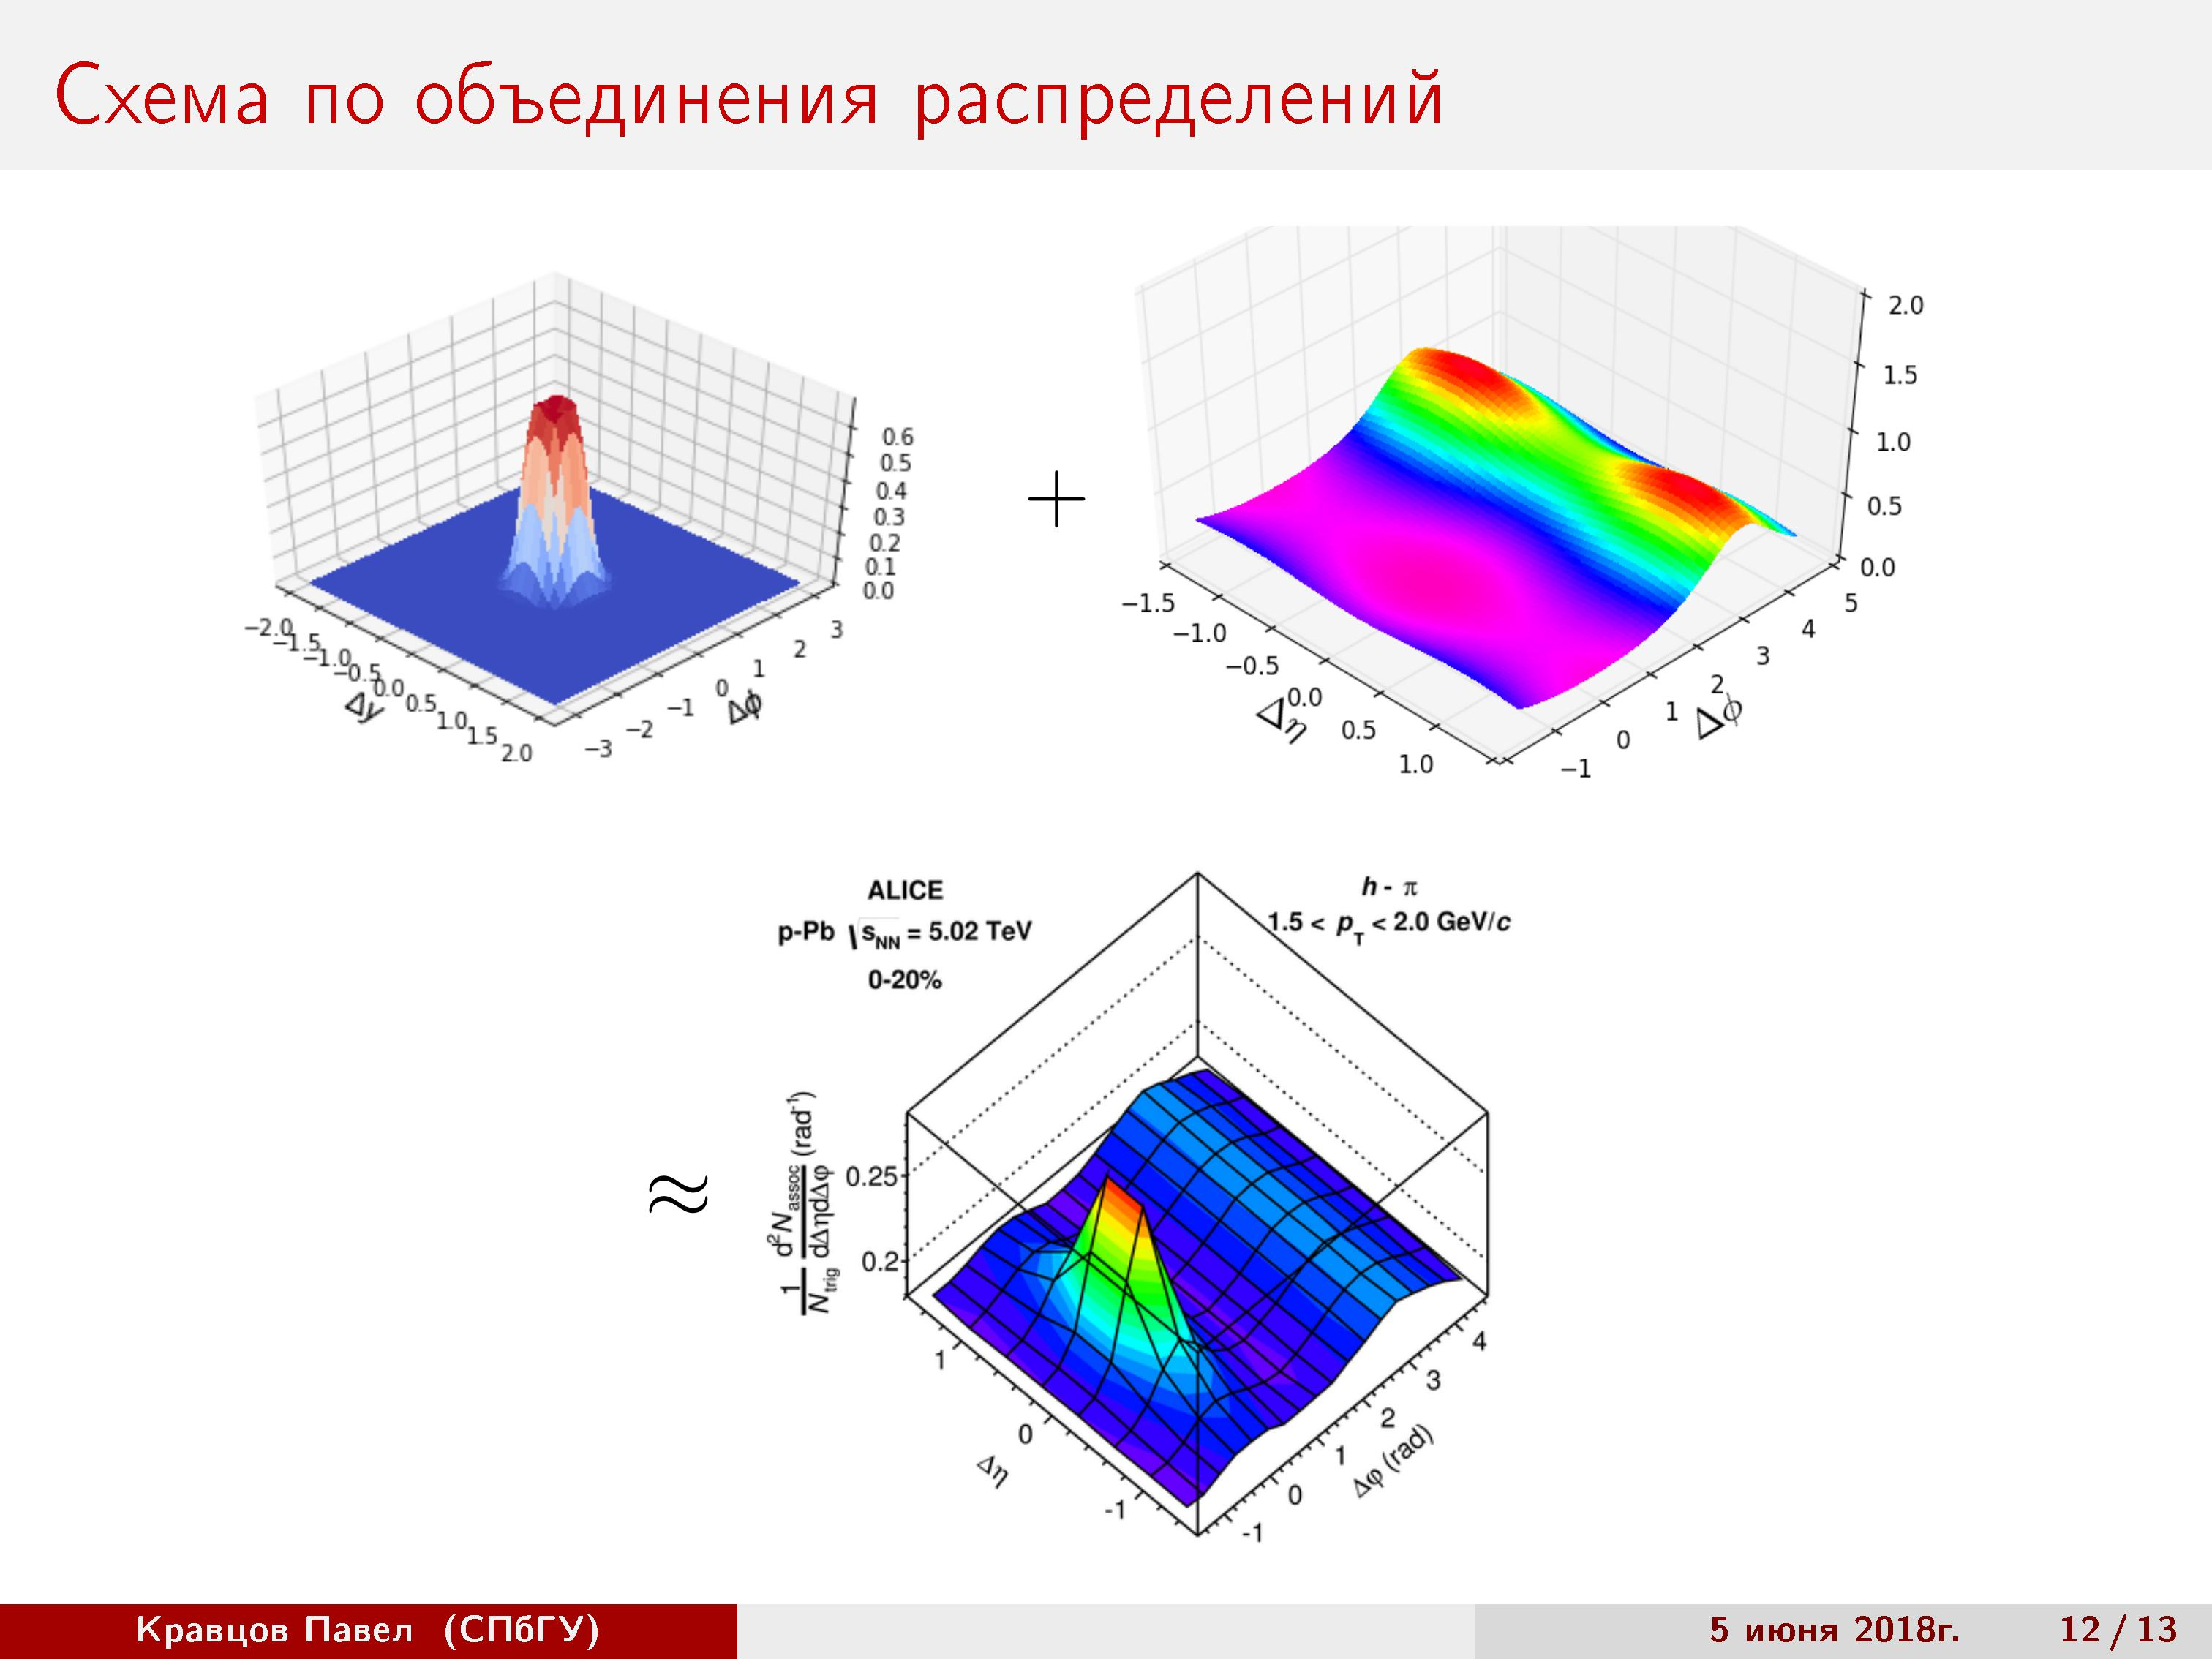
\includegraphics[width=1\linewidth]{page-12.jpg}
\end{minipage}
\begin{minipage}[h]{0.7\linewidth}
	От таких корреляций получаются 2 более низких и пологих пика вс центром $\phi = \pi, \Dy = \pm 1$. Они образуют структуру которая называется задний ридж. Если скомбинировать две простые модели, из этой работы и из бакалаврской, то они уже объясняют в общих чертах экспериментальные данные. Кроме того эту конструкцию можно улучшать добавляя различные эффекты, вроде слияния струн или учет поперечного импульса.
\end{minipage}
\line

\begin{minipage}[h]{0.29\linewidth}
	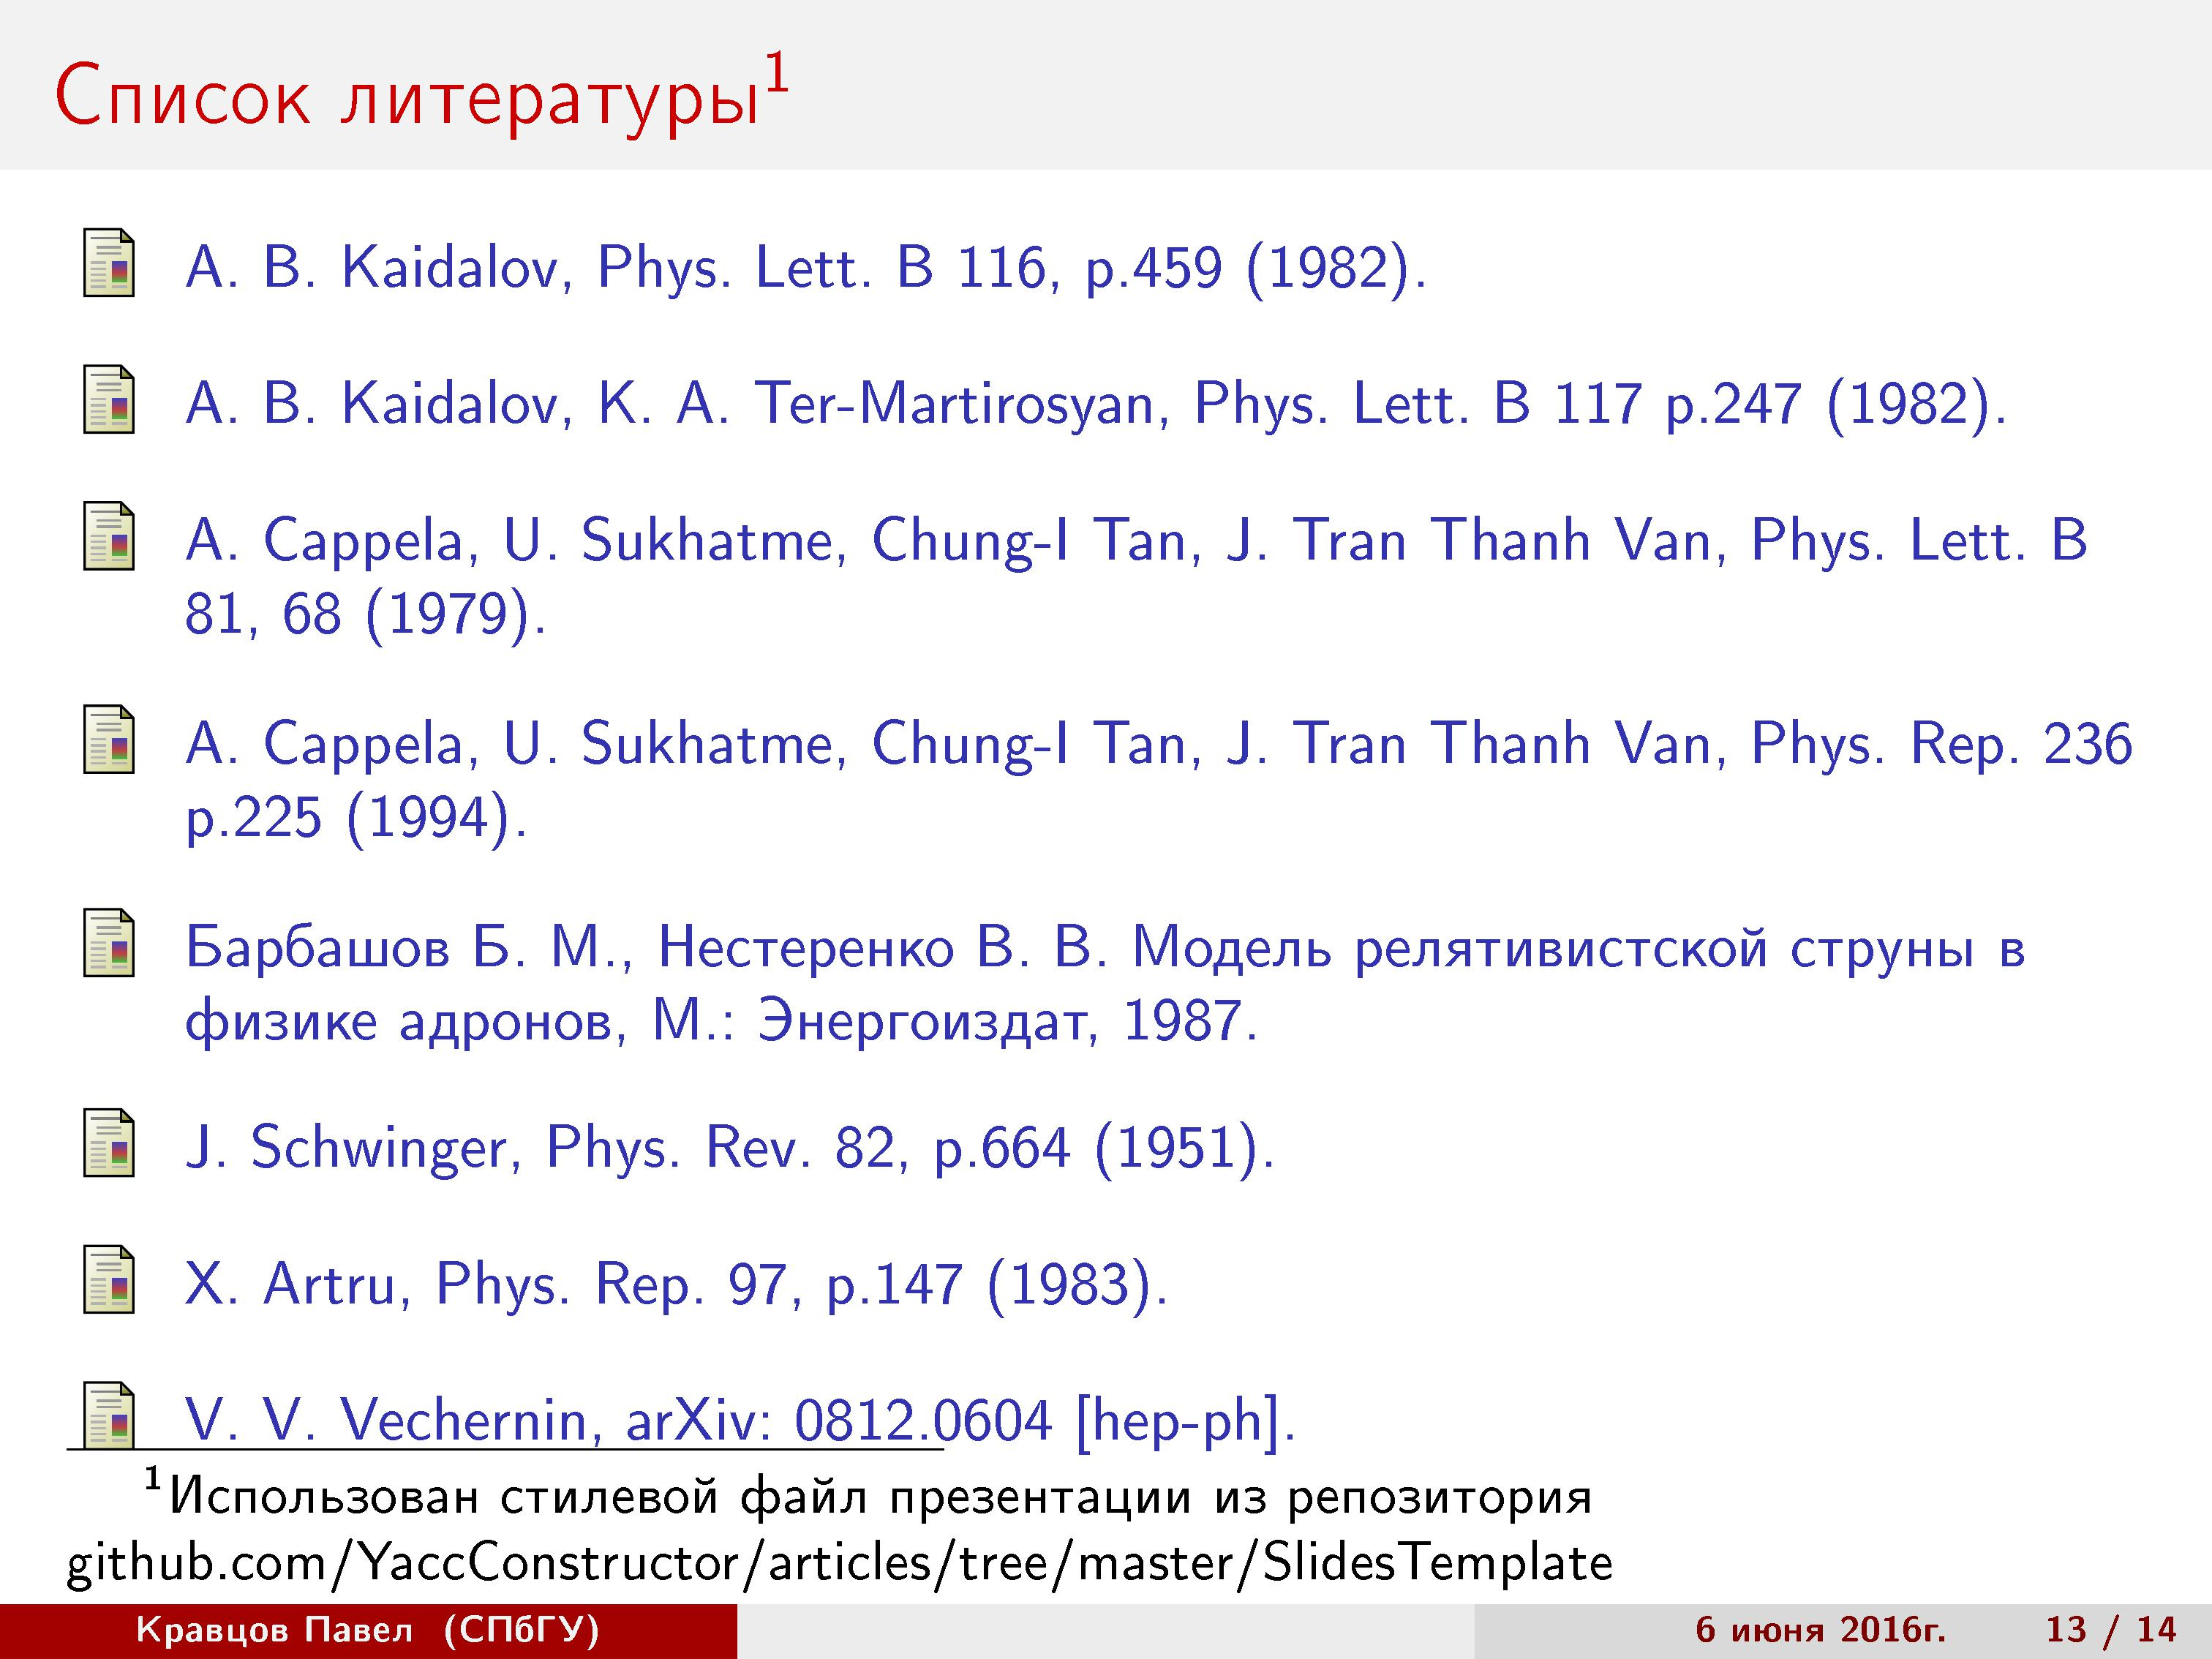
\includegraphics[width=1\linewidth]{page-13.jpg}
\end{minipage}
\begin{minipage}[h]{0.7\linewidth}
	Результаты работы: \\
	\qquad Была построена модель объясняющая образование переднего пика посредством влияния распада $\rho$-резонансов. Модель может использоваться как составная часть более сложных моделей. \\
	\qquad Для  $\rho (\Dy, \Dphi)$ удалось найти аналитическую формулу. Она может быть использованна для аппроксимации экспериментальных данных, нахождения параметров столкновения и их погрешностей. \\
	На этом все, спасибо за внимание.
\end{minipage}
\line

\end{document}